% Computer Science Tripos Part II project dissertation
\documentclass[12pt,a4paper,twoside,openany]{report}
\usepackage{fontspec}
\usepackage[
    backend=biber,
    natbib=true,
    style=ieee,
    url=false,
    doi=true
%eprint=false
]{biblatex}
\usepackage[pdfborder={0 0 0}]{hyperref}    % turns references into hyperlinks
\usepackage[margin=2cm,top=24mm,bottom=24mm]{geometry}  % adjusts page layout
\usepackage{graphicx}  % allows inclusion of PDF, PNG and JPG images
\usepackage{verbatim}
\usepackage{docmute}   % only needed to allow inclusion of proposal.tex
\usepackage{fancyvrb}
\usepackage[font=footnotesize,labelfont=bf]{caption}
\PassOptionsToPackage{obeyspaces}{url}
\usepackage{float}
\usepackage{enumitem}
\usepackage{changepage}
\usepackage{amsmath}
\usepackage{amssymb}
\usepackage{csquotes}
\usepackage[
    nottoc,
    notlot,
    notlof
]{tocbibind}
\usepackage{amsfonts}
\usepackage{mathtools}
\usepackage[dvipsnames]{xcolor}
\usepackage{cleveref}
\usepackage{tikz}
\usepackage{tabto}
\usepackage{xspace}
\usepackage{relsize}
\usepackage{bm}
\usepackage{bookmark}
\usepackage{listings}
\usepackage{fontawesome}
\usepackage{footnotehyper}
\usepackage{bashful}
\usepackage{dirtree}
\usepackage{pifont}
\usepackage{wrapfig}
\usepackage{graphbox}
\usepackage{tablefootnote}
%! Suppress = MultipleIncludes
\usepackage{afterpage}
\usepackage{hyphenat}
\usepackage{ragged2e}
\usepackage{array}
\usepackage{titlesec}
\usepackage{booktabs}
\usepackage{epigraph}
\usepackage{chngcntr}
\usepackage{subcaption}
\usepackage{mdframed}
\usepackage[bottom]{footmisc}

\usetikzlibrary{shadows.blur}

\newfontfamily\jbmono{JetBrainsMono}[
    Path = fonts/JetBrainsMono-1.0.3/ttf/,
    Extension = .ttf,
    NFSSFamily = jbmono,
    UprightFont = *-Regular,
    BoldFont = *-Bold,
    ItalicFont = *-Italic,
    BoldItalicFont = *-Bold-Italic,
    FontFace = {sb}{n}{*-Medium},
    FontFace = {sb}{it}{*-Medium-Italic},
    FontFace = {eb}{n}{*-ExtraBold},
    FontFace = {eb}{it}{*-ExtraBold-Italic},
    Scale = 0.87,
]
\renewcommand{\ttdefault}{jbmono}
\renewcommand*{\bibfont}{\small}

\addbibresource{refs.bib}
\graphicspath{{figures/}{figures_gen/}{images/}}

%TC:macro \cmt [ignore]
%TC:macro \url 1

% @formatter:off
\bash[stdoutFile=wordcount.tex]
texcount -1 -merge -q -utf8 -sum main.tex | tr -d '\n'
\END
% @formatter:on


\raggedbottom                           % try to avoid widows and orphans
\sloppy
\clubpenalty1000%
\widowpenalty1000%

% Spacing
\renewcommand{\baselinestretch}{1.08}    % adjust line spacing to make more readable
\setlength{\parskip}{2pt plus2pt minus1pt}
\titlespacing{\paragraph}{%
    \parindent}{%              left margin
    0pt}{% space before (vertical)
    1em}%               space after (horizontal)
\titlespacing*{\subsection}{0pt}{2.4ex plus 1.5ex minus .2ex}{1.2ex plus .4ex}
\titlespacing*{\subsubsection}{0pt}{2.2ex plus 1.5ex minus .2ex}{1.2ex plus .4ex}

%\titleformat{\chapter}[display]
%{\normalfont\huge\bfseries}{\chaptertitlename\ \thechapter}{20pt}{\Huge}
%\titlespacing*{\chapter}{0pt}{0pt}{30pt}

\titleformat{\chapter}[block]
{\normalfont\huge\bfseries}{\thechapter.}{1em}{\Huge}
\titlespacing*{\chapter}{0pt}{-19pt}{30pt}


%https://tex.stackexchange.com/questions/39017/how-to-influence-the-position-of-float-environments-like-figure-and-table-in-lat
\renewcommand{\floatpagefraction}{.8}%

% Better footnote handling
\newcounter{footnoteInText}
\newcounter{footnoteInNote}
\newcommand{\fnmark}{\stepcounter{footnoteInText}\setcounter{footnote}{\value{footnoteInText}}\addtocounter{footnote}{-1}\footnotemark{}}
\newcommand{\fntext}[1]{\stepcounter{footnoteInNote}\setcounter{footnote}{\value{footnoteInNote}}\footnotetext{#1}}

\setcounter{tocdepth}{3}
\setcounter{secnumdepth}{4}
\counterwithout{footnote}{chapter}
\allowdisplaybreaks


%! Suppress = PrimitiveStyle
%! Suppress = DiscouragedUseOfDef
%! Suppress = Makeatletter

% Definition

\makeatletter
\def\@begintheorem#1#2{\trivlist
    \item[\hskip \labelsep{\bfseries #1\ #2}]\mbox\newline\quote\itshape}
\def\@opargbegintheorem#1#2#3{\trivlist
    \item[\hskip \labelsep{\bfseries #1\ #2\ (#3)}]\mbox\newline\quote\itshape}
\def\@endtheorem{\endquote\endtrivlist}
\makeatother

\newtheorem{definition}{Definition}[section]
\newcommand*{\definitionautorefname}{Definition}

% References
\crefformat{footnote}{#2\footnotemark[#1]#3}

% Math mode
\newcommand{\Set}[2]{\left\{\, #1 \mid #2 \, \right\}}
\newcommand\eqdef{\ \,\stackrel{\mathclap{\normalfont\mbox{def}}}{=}\,\ }
\newcommand\generates[1]{\ \,\overset{#1}{\hookrightarrow}\,\ }
\newcommand\integersto[1]{\left\{1, \dots, #1\right\}}
\DeclareMathOperator{\ego}{ego}

% Snippets
\newcommand{\citeneeded}{\colorbox{Apricot}{[?]}}
\newcommand{\todo}[1]{\colorbox{GreenYellow}{TODO: #1}}
\newcommand{\unimportant}[1]{\textcolor[rgb]{0.6,0.6,0.6}{#1}}

\newcommand{\graffs}{\texttt{graffs}\xspace}
\newcommand{\parspace}{\bigskip}

% Lists
\setlist[itemize]{itemsep=0pt}

\newlist{todolist}{itemize}{2}
\setlist[todolist]{label=$\square$}
\newcommand{\done}{\rlap{$\square$}{\raisebox{2pt}{\large\hspace{1pt}\ding{51}}}\hspace{-2.5pt}}
%\newcommand{\wontfix}{\rlap{$\square$}{\large\hspace{1pt}\ding{55}}}

% Figures
\makeatletter
\g@addto@macro\@floatboxreset\centering
\makeatother

% Directory trees
\def\FTdir(#1,#2,#3){%
    \FTfile(#1,{{\color{black!40!white}\faFolderOpen}\hspace{0.2em}#3})
    (tmp.west)++(0.8em,-0.4em)node(#2){}
    (tmp.west)++(1.5em,0)
    ++(0,-1.3em)
}
\def\FTfile(#1,#2){%
    node(tmp){}
    (#1|-tmp)++(1.0em,0)
    node(tmp)[anchor=west,black]{\tt\fontsize{10pt}{10pt}\selectfont #2}
    (#1)|-(tmp.west)
    ++(0,-1.2em)
}
\def\FTroot{tmp.west}

% Code listing
\makeatletter
\newcommand*\idstyle{%
    \expandafter\id@style\the\lst@token\relax
}
\def\id@style#1#2\relax{%
    \ifcat#1\relax\else
    \ifnum`#1=\uccode`#1%
    \bfseries\color{black}
    \fi
    \fi
}
\makeatother

\lstdefinelanguage{Kotlin}{
    comment=[l]{//},
    commentstyle={\color{gray}\ttfamily},
    emph={delegate, filter, first, firstOrNull, forEach, lazy, map, mapNotNull, println, return@},
    emphstyle={\color{OrangeRed}},
    identifierstyle=\idstyle,
    keywords={abstract, actual, as, as?, break, by, class, companion, continue, data, do, dynamic, else, enum, expect, false, final, for, fun, get, if, import, in, interface, internal, is, null, object, override, package, private, public, return, set, super, suspend, this, throw, true, try, typealias, val, var, vararg, when, where, while},
    keywordstyle={\color{NavyBlue}\bfseries},
    morecomment=[s]{/*}{*/},
    morestring=[b]",
    morestring=[s]{"""*}{*"""},
    ndkeywords={@Deprecated, @JvmField, @JvmName, @JvmOverloads, @JvmStatic, @JvmSynthetic, Array, Byte, Double, Float, Int, Integer, Iterable, Long, Runnable, Short, String, @Entity, @ManyToOne, @ElementCollection, @OneToMany, @LazyCollection},
    ndkeywordstyle={\color{BurntOrange}\bfseries},
    sensitive=true,
    stringstyle={\color{ForestGreen}\ttfamily},
}

\let\origthelstnumber\thelstnumber
\makeatletter
\newcommand*\Suppresslinenumbers{%
    \lst@AddToHook{OnNewLine}{%
    %! Suppress = DuplicateDefinition
        \let\thelstnumber\relax%
        \advance\c@lstnumber-\@ne\relax%
    }%
}
\newcommand*\Reactivatelinenumbers{%
    \lst@AddToHook{OnNewLine}{%
    %! Suppress = DuplicateDefinition
        \let\thelstnumber\origthelstnumber%
        \advance\c@lstnumber\@ne\relax}%
}
\lstdefinestyle{light}{%
    basicstyle=\ttfamily\color{black},
    breaklines=true,
    frame=none,
    numbers=none,
    xleftmargin=2\parindent,
}
\lstset{%! Suppress = NonMatchingIf
    basicstyle=\ttfamily\color{black}\lst@ifdisplaystyle\fontsize{10pt}{10pt}\selectfont\fi,
    belowcaptionskip=8pt,
    breaklines=true,
    escapechar=¦,
    frame=single,
    includerangemarker=false,
    inputpath=listings/,
    numbers=left,
    numbersep=6pt,
    numberstyle=\fontsize{7pt}{7pt}\selectfont\color{gray},
    rangeprefix=//-----,rangesuffix=-----,
    showspaces=false,
    showstringspaces=false,
    tabsize=1,
}
\makeatother

\lstMakeShortInline[columns=fixed]|


\begin{document}
    %TC:ignore

    %%%%%%%%%%%%%%%%%%%%%%%%%%%%%%%%%%%%%%%%%%%%%%%%%%%%%%%%%%%%%%%%%%%%%%%%
    % Title

    \pagestyle{empty}

    \begin{minipage}{.45\linewidth}
        \begin{flushleft}
            
\includegraphics[height=10mm]{uc-black-white.eps}
        \end{flushleft}
    \end{minipage}
    \hfill
    \begin{minipage}{.45\linewidth}
        \begin{flushright}
            \Large \textbf{Juraj Mi\v{c}ko} \\
            \normalsize \href{mailto:jm2186@cam.ac.uk}{jm2186@cam.ac.uk}
        \end{flushright}
    \end{minipage}

    \vspace*{45mm}
    \begin{center}
        \LARGE
        \textbf{Framework for Empirical Analysis of Graph Metric Robustness} \\[5mm]

        \vspace{5mm}
        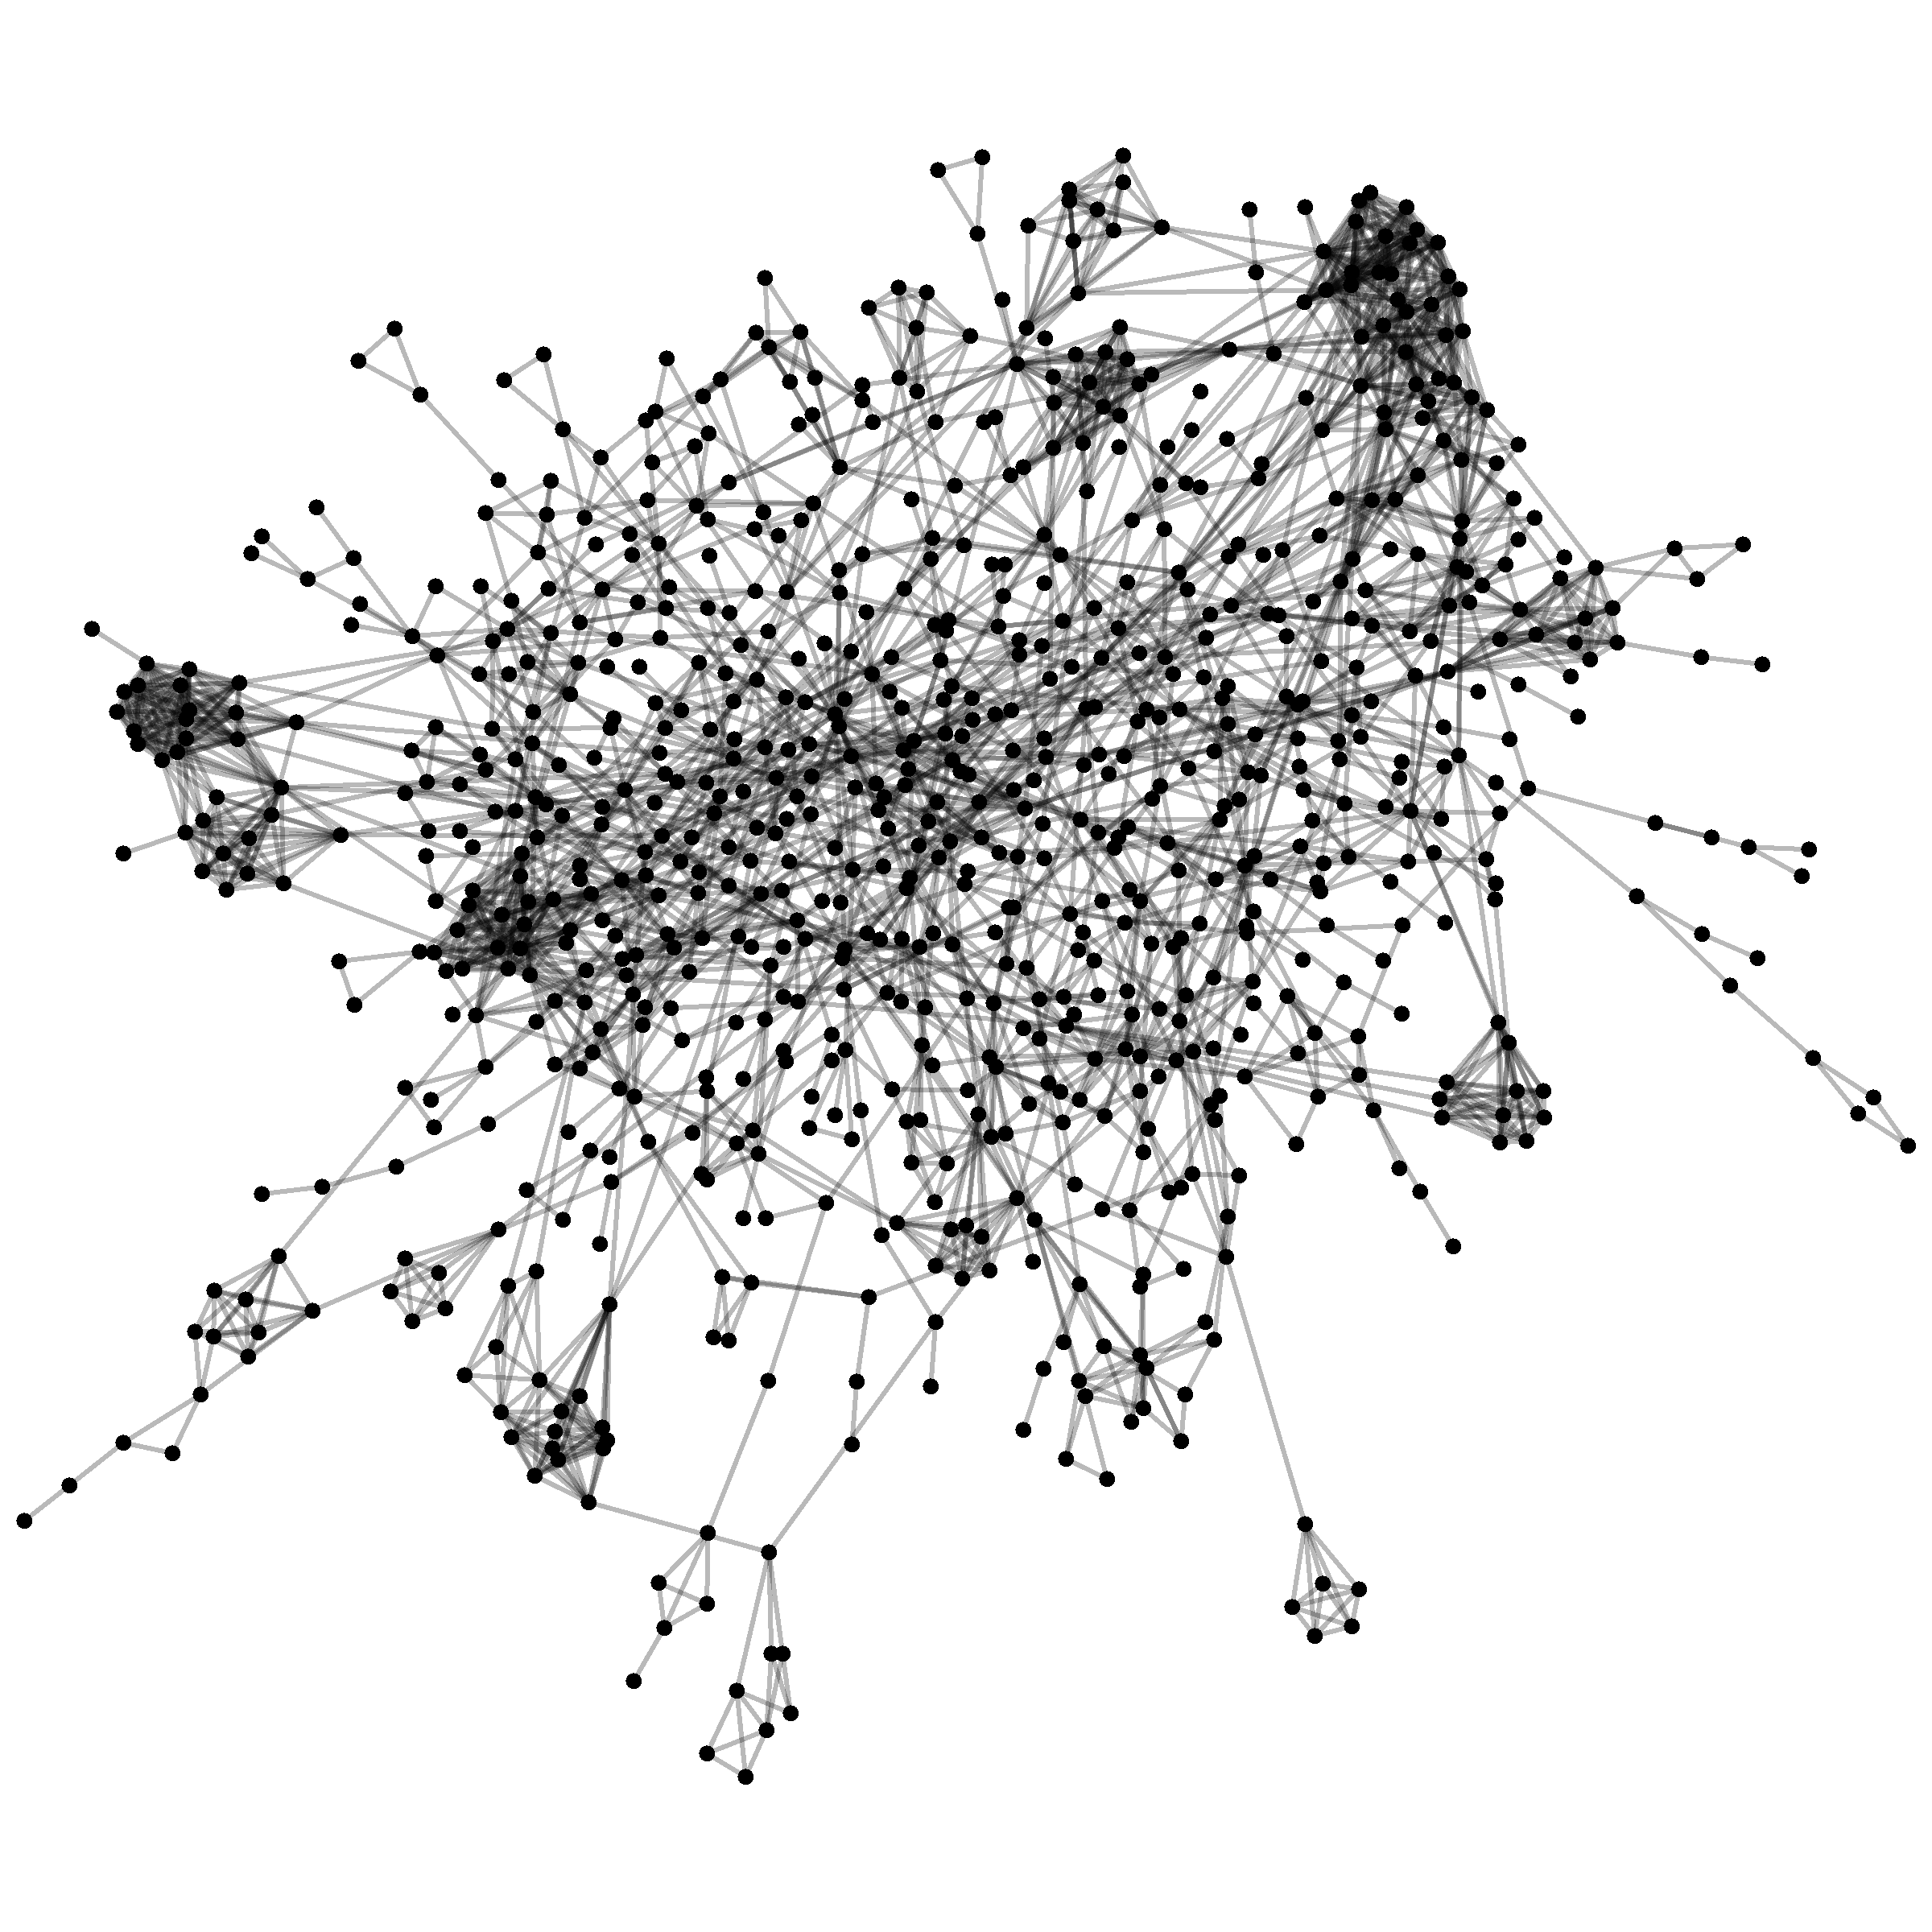
\includegraphics[height=9cm]{cover_graph_img.png}
        \vspace{5mm}

        \Large
        Jesus College \\
        University of Cambridge \\[5mm]
        Computer Science Tripos -- Part II \\[5mm]
        \today  % today's date
    \end{center}

    \clearpage

    %%%%%%%%%%%%%%%%%%%%%%%%%%%%%%%%%%%%%%%%%%%%%%%%%%%%%%%%%%%%%%%%%%%%%%%%%%%%%%
    % Proforma, table of contents and list of figures

    \pagenumbering{roman}
    \pagestyle{plain}
    \chapter*{Declaration}

    I, Juraj Mi\v{c}ko of Jesus College, being a candidate for Part II of the Computer Science Tripos, hereby declare that this dissertation and the work described in it are my own work, unaided except as may be specified below, and that the dissertation does not contain material that has already been used to any substantial extent for a comparable purpose.

    \bigskip
    \noindent
    I, Juraj Mi\v{c}ko of Jesus College, am content for my dissertation to be made available to the students and staff of the University.

    \vspace{1cm}\noindent
    \begin{tabular}{@{}l@{\hspace{2\tabcolsep}}l}
        Signed: & \hspace*{2mm}
\includegraphics[width=28mm]{signature.png}\vspace{-1mm}\hspace*{2mm} \\
        \cline{2-2}
        & \multicolumn{1}{r}{\textit{Juraj Mi\v{c}ko}} \\[3mm]
        Date: & \today
    \end{tabular}


    \newpage
    \chapter*{Proforma}

    {\large
        \begin{savenotes}
            \begin{tabular}{ll}
                Candidate number: & \textbf{2343F}                            \\
                Project Title: & \textbf{Framework for Empirical Analysis} \\ & \textbf{of Graph Metric Robustness}                    \\
                Examination: & \textbf{Computer Science Tripos -- Part II, 2020} \\
                Word Count: & \textbf{\input{wordcount.tex}\footnote{This word count was computed using: \texttt{texcount -1 -merge -q -utf8 -sum main.tex}}}                                    \\
                Line Count: & \textbf{5694} \footnote{This total lines of code count was computed using:\verbatiminput{count-lines.sh} } \\
                Project Originator: & \textbf{Dr Timothy Griffin}                               \\
                Supervisor: & \textbf{Dr Timothy Griffin}                                        \\
            \end{tabular}
        \end{savenotes}
    }

    \section*{Original aims of the project}

    Networks are commonly analysed using graph metrics to identify their key properties.
    However, real-world data can be inherently imprecise, leading to inaccuracies in the measured metric values.
    A paper by Bozhilova et al.~\cite{Bozhilova2019} tackles a similar problem, quantifying robustness of metrics in scored protein interaction networks.

    The project will first follow their experimental approach to produce similar results.
    Second, it will extend the concept of rank robustness of metrics to unscored networks, studying how susceptible they are to small perturbations in graphs.
    The result will be a tool that facilitates experiments of measuring robustness of metrics on many network datasets.


    \section*{Work completed}

    I designed a way to analyse robustness of graph metrics on unscored networks, advancing the concept of rank robustness from the paper by Bozhilova et al.
    I built a command-line tool \graffs from scratch in Kotlin, for carrying out large-scale computation-heavy experiments of measuring robustness of metrics, in an efficient, flexible, and reproducible way.
    I set up a high-performance computing environment and reproduced expected results as well as derived new interesting results.

    The project met all success criteria.
    As an extension, I proposed further research within this novel field and published \graffs as open-source, ready to be reused and extended.


    \section*{Special difficulties}

    Due to world-wide measures related to the COVID-19 pandemic, I was held in Azerbaijan for 6 weeks, uncertain about possible repatriation travels, then spent two weeks in a compulsory government quarantine facility and in self-isolation in Slovakia, before returning home to a working environment.

    I was approved a two-week extension which largely accounted for these circumstances, and had no other special difficulties.


    \tableofcontents
    \clearpage

    %\listoffigures
    %\listoftables
    %\lstlistoflistings

    %%%%%%%%%%%%%%%%%%%%%%%%%%%%%%%%%%%%%%%%%%%%%%%%%%%%%%%%%%%%%%%%%%%%%%%
    % now for the chapters

    \pagenumbering{arabic}
    \pagestyle{headings}

    %TC:endignore
    \chapter{Introduction}\label{ch:introduction}
    I designed a way and built a tool to analyse robustness of graph metrics.

\section{Motivation}

This project was inspired by, and is based on the following paper~\cite{Bozhilova2019} (further referred to as ``The Paper'') which served as a kickoff point for this project.
\begin{adjustwidth}{1cm}{}
    \vspace*{0.5em}
    Bozhilova, L. V., Whitmore, A. V., Wray, J., Reinert, G., \& Deane, C. M. (2019). Measuring rank robustness in scored protein interaction networks. BMC Bioinformatics, 20(1). \url{https://doi.org/10.1186/s12859-019-3036-6}
    \vspace*{0.5em}
\end{adjustwidth}

Graph metrics are often used to find and derive facts about important nodes or components of networks.
However, real-world datasets may be inherently imprecise, or the procedure of obtaining networks from raw measured data may introduce (sometimes invisible) inaccuracies.
When evaluating graph metrics on imprecise data, it is crucial to be able to reason about the reliability and of the results, as with any other statistical procedures.

The Paper introduces ways to assess \textsl{robustness} of graph metrics specifically on protein interaction networks with confidence-scored edges.

I built a tool that can measure robustness of graph metrics on any graph dataset, extending the idea from The Paper to networks with unweighted edges.

\section{Graphs}

%The total data (created, captured or replicated) in the world by 2018 was estimated to be 18 zettabytes in 2018 and is expected to reach 175 zettabytes by 2025~\cite{ReinselDigitizationWorldEdge2018}.
Ever-increasing data sources and applications of data science force researchers and data scientists to use tools such as graph theory to model real-world problems.
Graphs, or networks (nodes and edges), can capture many types of entities and their relations in the real world.
Graph theory, believed to have been invented by L. Euler in 18th century~\cite{BiggsGraphTheory173619361986} has been since used to help solve problems in the field of information technology, engineering, biology, chemistry, social systems, geography, linguistics and many more ~\cite{FouldsGraphTheoryApplications2012}.
A simple example is a social network in which nodes may represent people and edges represent existence of relationships between pairs of people.


\section{Graph metrics}

Graph theory proved especially useful when analysing large structures of data that cannot simply be visualised or otherwise analysed by investigating individual entities.
The word \textsl{network} is often used in this context to refer to large instances of graphs stemming from real systems, as opposed to graphs referring more to the mathematical concept itself.
Graph \textsl{statistics} (e.g. size, average degree, diameter, radius) have been invented to help mathematically describe properties of arbitrarily large graphs, such as betweenness centrality.
Further, graph \textsl{metrics} (such as betweenness centrality, closeness centrality, eccentricity) quantify properties of individual nodes.
For example a person represented by a node with high closeness centrality score is considered to be \textsl{closer} to others in terms of number of hops needed, in other words can spread information in the network faster.

Protein interaction networks is an example of a prominent research field relying on graph theory.
Nodes in protein networks represent proteins present in cells of organisms and edges represent interactions between them, possibly labelled to convey additional information.
Studying such networks helps in understanding physiology of biological cells and developing drugs as they generally affect protein interactions.


\section{Imperfect data}

The problem is, networks constructed from real-world contain errors such as missing nodes or edges, false positives, uncertain nodes or edges, falsely aggregated nodes.
Network errors may stem from measurement errors, approximations, lack of knowledge, lack of experimental evidence or thresholding of scored networks~\cite{Wang2012,MarsdenNetworkDataMeasurement1990,JonesChallengesLimitationsQuantifying2010}.
These errors may then propagate and cause errors in graph metrics, which the user of the dataset may not be aware of. \todo{clarify}

For example, the STRING database\cite{Szklarczyk2019} is an open collection that contains known and predicted protein-protein interactions.
It provides confidence scores for edges, indicating how likely the dataset authors consider an interaction to be true, given the available evidence.
The Paper~\cite{Bozhilova2019} demonstrates instability of some graph metrics on thresholded protein networks and proposes ways to assess robustness of graph metrics in such networks.


\section{Metric robustness}

Although the field of investigating graph metric robustness is novel and recent, a number of attempts tried to assess robustness or stability properties of graph metrics.
Examples are analysing impact of errors on centrality measures in random networks~\cite{BorgattiRobustnessCentralityMeasures2006} or, more specifically, evaluating reproducibility of metrics on multi-temporal scans of human brain using coefficient of variation (CV), the repeatability coefficient (RC) and the intra class correlation (ICC)~\cite{VaessenEffectReproducibilityDifferent2010,DennisTestRetestReliabilityGraph2012}.
A significant amount of research analysing reproducibility of metrics in uncertain brain networks appeared around 2011, summarised in~\cite{TelesfordExplorationGraphMetric2013}.
The latest research led to development of methods for analysis of such uncertain data, estimating a ground-truth network structure from imperfect data~\cite{Martin2016,Newman2018}, and even a method to mitigate sensitivity of metrics on the selection of a threshold in scored networks~\cite{Drakesmith2015}.

One of the most recent researches on metric robustness is already mentioned work on protein interaction networks in The Paper.
In the study they use 3 ways to quantify metric robustness, focusing on comparing node rankings induced by each metric at different score thresholds instead of the calculated values, arguing that comparing ranks better assesses robustness of metrics.
Those robustness measures are: Rank continuity (comparing sets of highly ranked nodes between graphs derived from similar confidence threshold), Rank identifiability (considering overall ranks of all nodes and quantifying how much these ranks differ from ranks observed in graphs derived from various confidence thresholds), Rank instability (quantifying variation of ranks of top 1\% of nodes over a certain confidence range).


\section{Software tool: \graffs}

\todo{revise once done}

In this dissertation I summarise the research done on this topic and build a command-line tool that helps generalise the research of graph metric robustness and allows application of the above mentioned methods to graphs of other kinds.
\Cref{ch:preparation} explains The Paper in more detail, revises the background material and proposes the method used in the framework.

First, I generalise graph acquisition using different methods on different source datasets, such as edge score thresholding or random edge removal.
Consequently, the framework applies a number of robustness measures on some of the most common node-level graph metrics, and tries to infer any correlation between graph classes and robustness of metrics used on them.
\Cref{ch:implementation} describes the framework implementation of the framework, which I then evaluate in \cref{ch:evaluation}.

\todo{describe evaluation?}


I wrapped up the project named \graffs and published it as an open-source library that can further be used by future projects in this research area.



    \chapter{Preparation}\label{ch:preparation}
    In this chapter I explain my preparatory work, which mainly consists of understanding the problem from the mathematical and research point of view.
First, I explain in detail why measuring robustness of graph metrics is an important and a novel field, describing in detail the work done in ``The Paper'' that this dissertation is based on.
Further I introduce specific definitions of graph metrics and robustness measures that I use in the implementation.


\section{Introduction to confidence}

Statistical significance, confidence scores, confidence intervals, error ranges, all are used to signal or approximate the extent to which the observed result is reliable.
Some of the confidence values are a direct probability that an error is made, given the available evidence, such as a statistical significance when rejecting a null hypothesis, or confidence intervals.
Other error values such as error ranges or standard deviations estimate how much off a numerical value may be.
These error measures are all important to state and assess how precise or confident an experiment or an observation is.

A research result without assessing its precision or confidence can be considered incomplete.
We need the assessment of possible error to derive any further guidance from the research.\citeneeded

However, can we measure the precision, or the confidence or graph metrics?
If research is based on evaluating metrics on graphs which are themselves imprecise or having possible errors in the structure, how can we assess the confidence or precision of such result?


\section{The Paper}

This dissertation project is based on, and extending the ideas from the paper by Bozhilova et al.: \textsl{Measuring rank robustness in scored protein interaction networks}\cite{Bozhilova2019}.
From now on, I will refer to it as \textsl{The Paper}.

\subsection{Protein networks}

Protein networks is a large research field with a plethora of uses, and investigating them is important for the future of bioinformatics~\todo{examples + citations}.

Most graph datasets obtained from the real-world, including protein interaction networks (PINs), are a result of experiments or observations which possibly introduce measurement errors, either systematic or random errors.

Also, protein networks have a specific structure: nodes represent proteins and weighted (or scored) edges represent the presence of interactions between proteins.
It is assumed that such interactions are mutual, therefore the formed graph is undirected.

\begin{figure}[ht]
    \vspace*{-3mm}
    \tikzset{every picture/.style={line width=0.75pt}} %set default line width to 0.75pt
    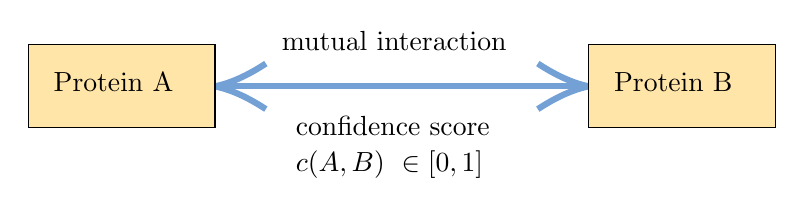
\begin{tikzpicture}[x=0.75pt,y=0.75pt,yscale=-1,xscale=1]
        %uncomment if require: \path (0,136); %set diagram left start at 0, and has height of 136

        %Straight Lines [id:da5202946805882411]
        \draw [color={rgb, 255:red, 115; green, 161; blue, 213 }  ,draw opacity=1 ][fill={rgb, 255:red, 0; green, 0; blue, 0 }  ,fill opacity=1 ][line width=2.25]    (114,40) -- (286,40) ;
        \draw [shift={(290,40)}, rotate = 180] [color={rgb, 255:red, 115; green, 161; blue, 213 }  ,draw opacity=1 ][line width=2.25]    (24.48,-10.98) .. controls (15.57,-5.15) and (7.41,-1.49) .. (0,0) .. controls (7.41,1.49) and (15.57,5.15) .. (24.48,10.98)   ;
        \draw [shift={(110,40)}, rotate = 0] [color={rgb, 255:red, 115; green, 161; blue, 213 }  ,draw opacity=1 ][line width=2.25]    (24.48,-10.98) .. controls (15.57,-5.15) and (7.41,-1.49) .. (0,0) .. controls (7.41,1.49) and (15.57,5.15) .. (24.48,10.98)   ;
        %Shape: Rectangle [id:dp8315683426496481]
        \draw  [fill={rgb, 255:red, 255; green, 229; blue, 168 }  ,fill opacity=1 ] (20,20) -- (110,20) -- (110,60) -- (20,60) -- cycle ;
        %Shape: Rectangle [id:dp6227729030936355]
        \draw  [fill={rgb, 255:red, 255; green, 229; blue, 168 }  ,fill opacity=1 ] (290,20) -- (380,20) -- (380,60) -- (290,60) -- cycle ;

        % Text Node
        \draw (31,32) node [anchor=north west][inner sep=0.75pt]   [align=left] {Protein A};
        % Text Node
        \draw (301,32) node [anchor=north west][inner sep=0.75pt]   [align=left] {Protein B};
        % Text Node
        \draw (141,12) node [anchor=north west][inner sep=0.75pt]   [align=left] {mutual interaction};
        % Text Node
        \draw (141,50.4) node [anchor=north west][inner sep=0.75pt]    {$ \begin{array}{l}
                                                                              \text{confidence score}\\
                                                                              c( A,B) \ \in [ 0,1]
        \end{array}$};
    \end{tikzpicture}
    \caption{Schematic of an interaction between two proteins}
    \vspace*{-2mm}
\end{figure}


\subsection{Confidence scores}

The weight of each edge represents a confidence score which may be a value, or a set of values, describing some sort of \textsl{likelihood} that the given interaction is true, given the available evidence.
They do \textsl{not} indicate the strength or intensity of the interaction (which would be a different property, usually not observed in such protein networks).

For example, in the STRING database of protein networks used in The Paper, the main interaction score is an approximated \textsl{confidence} based on evidence such as scientific experiments, genetic observations (gene fusions, gene co-occurrence), statistical predictions, text mining of scientific articles, or existing knowledge (other available protein interaction databases)~\cite{Szklarczyk2019}.
The database then contains score values for each type of evidence, as well as a combined overall confidence score.
The Paper, as well as my dissertation, use only the combined confidence score and do not focus on the biological details of each evidence type.

\begin{figure}
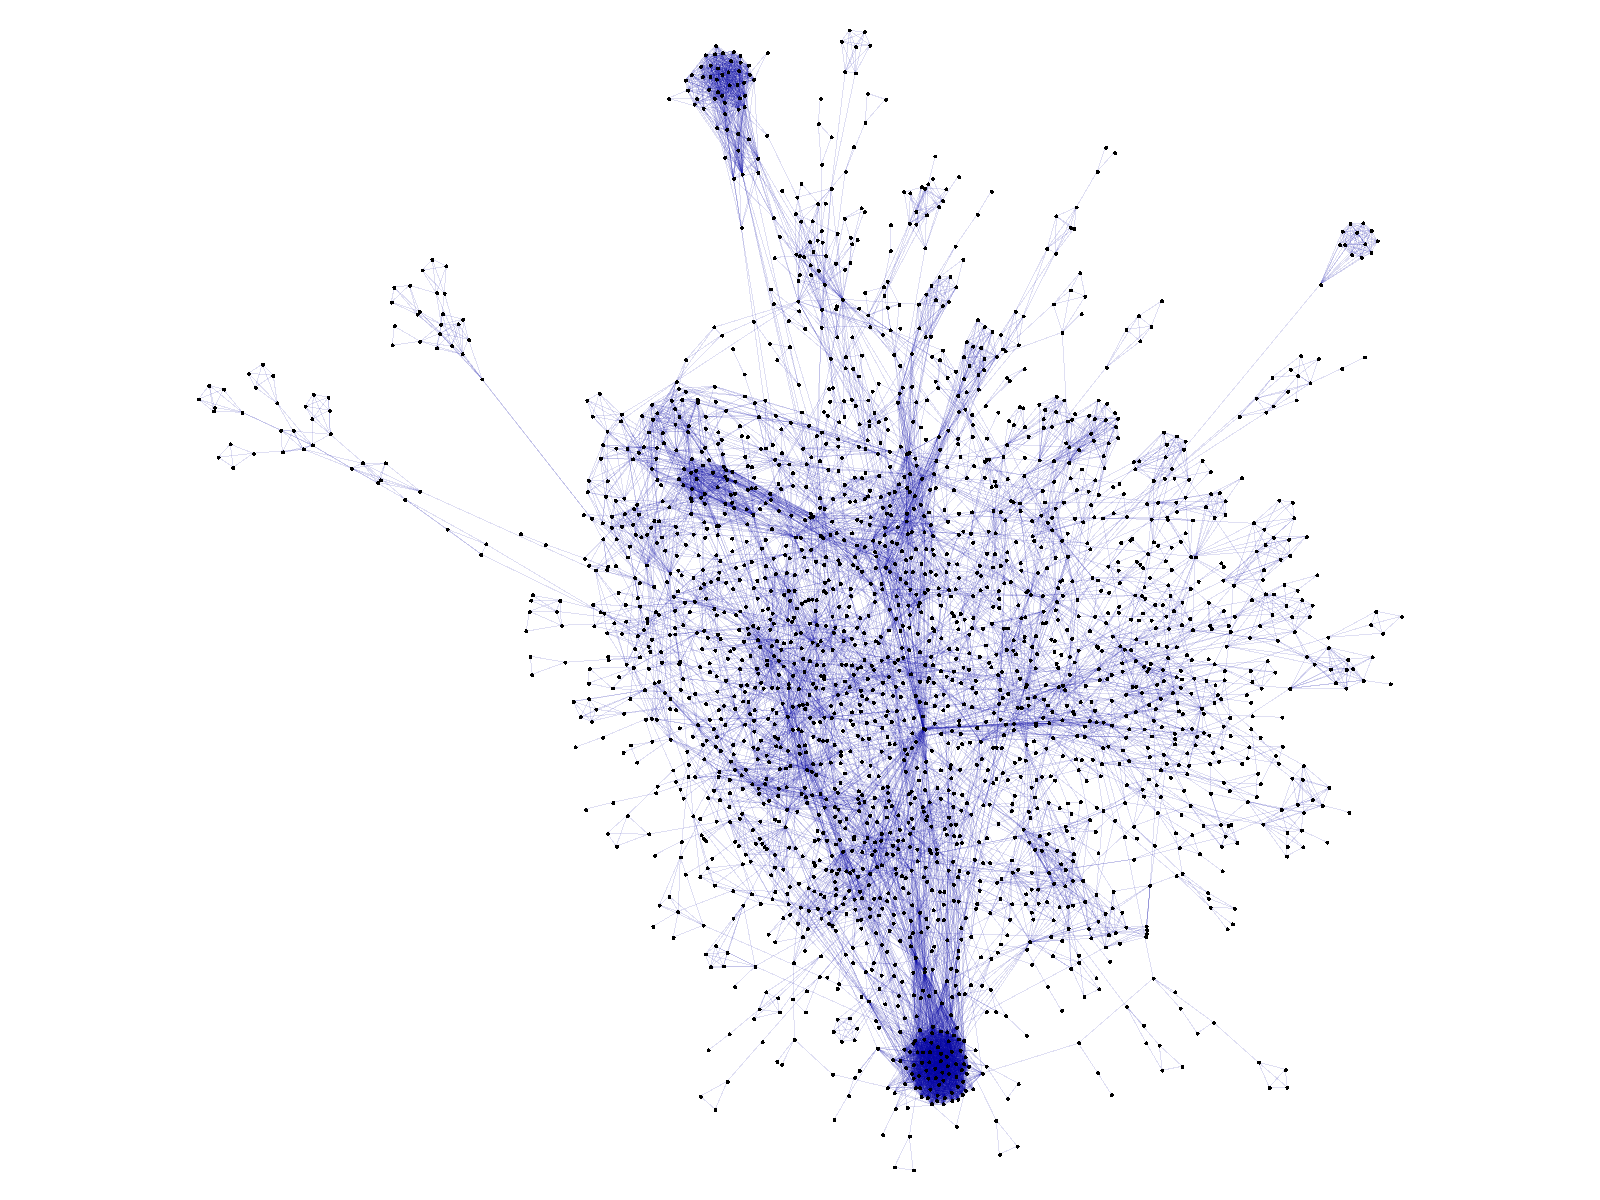
\includegraphics[height=8cm]{ecoli_giant_at_900.png}
\caption{An interaction network of proteins from the \textit{Escherichia coli} organism from the STRING database, thresholded at the $0.9$ score (high confidence). Only nodes of the giant component are shown.}
\label{fig:ecoli_giant_at_900}
\end{figure}


When researching protein interactions, in practice, researchers choose a \textbf{threshold} and then form a protein interaction network from the database considering only interactions (edges) whose confidence score is greater than the selected threshold, to only take into account interactions of sufficiently high quality.
Researchers then use tools such as graph metrics to identify important nodes or components of graphs, calculate statistics, or derive other results.

\autoref{fig:ecoli_giant_at_900} shows an example of a protein network taken from the STRING database\cite{Szklarczyk2019}, of proteins of the \textit{Escherichia coli} organism.
Only edges with score of $0.9$ corresponding to the ``highest confidence'' level (on the scale from $0$ to $1$) were retained, and only the giant connected component of it is shown.
That yields a graph with 2382 nodes and 12071 edges.

\subsection{Metric robustness}

However, as The Paper remarks, the analysis based on metric evaluation can be sensitive to the choice of the threshold.
If a node metric is to be useful for extracting biological signal, it should lead to similar results across networks obtained at different reasonable confidence score thresholds.
Hence, the point of studying metric robustness or \textsl{stability} is a way to assess how reliable the results are on a graph derived from a given threshold.

It is clear that numerical values of node metrics will depend on such threshold, for example the degree and the clustering coefficient of each node will indeed monotonically decline with declining density of the network, which monotonically declines as we increase the confidence threshold.
For this reason, the point of The Paper is to assess a robustness of graph metrics based on the \textbf{rankings} of nodes induced by each metric (where ranking is just a total preorder of the nodes based on the metric values).

\subsubsection{Rank robustness}

The Paper introduces three different measures assessing robustness of node metrics (all will be explained later):
\begin{itemize}
    \item rank continuity,
    \item rank identifiability,
    \item rank instability.
\end{itemize}
All three measures are based on rankings of nodes induced by node metrics, and not on the exact values, to mitigate the density bias described above.

The Paper studies robustness of 25 different \textsl{node} metrics only, i.e. graph metrics which return one numerical value per node.


\section{Mathematical background}

In this section I review background material on graph theory and examining graph metric robustness, and fix terms I will use later to avoid ambiguity in further chapters.

In particular, this section will focus introducing high-level concepts of:
\begin{itemize}
    \item relevant bits of graph theory
    \item graph metrics
    \item ranking
    \item metric robustness
\end{itemize}

\subsection{Graphs}

Graphs (or networks) from graph theory usually consist of \textit{components} (or nodes, vertices) and \textit{links} between them (edges).
Some definitions in this subsection are based on the book \textsl{A first course in network theory}\cite{Estrada2017}.

\begin{definition}[Graph]
    Let $V$ be a finite set of $n$ nodes (or vertices), and let $E \subseteq V \times V$ be a set of edges.\\
    A \textbf{graph} $G$ is a pair $(V, E)$.\\
    $V$ is the \textbf{node set} of $G$, and $E$ is the \textbf{edge set} of $G$.
\end{definition}

Real-world data (or datasets) in the form of graphs are also called \textbf{networks}.
Still, I may interchange the words \textsl{graph}, \textsl{network} and \textsl{dataset}, but generally:
\begin{itemize}
    \item \textsl{dataset} is data stored in its raw form, such as a file downloaded from the Internet
    \item \textsl{network} is the real-world graph-like data conveyed by a dataset
    \item \textsl{graph} is a hypothetical structure, also a mathematical interface or representation that algorithms work with
\end{itemize}

\begin{definition}[Graph properties]
    \begin{itemize}[leftmargin=*]
        \item $G$ is \textbf{reflexive} iff $\forall v \in V.\ (v, v) \in E$
        \item $G$ is \textbf{anti-reflexive} iff $\forall v \in V.\ (v, v) \notin E$
        \item $G$ is \textbf{undirected} (or equally \textbf{symmetric}) iff $\forall v_1, v_2 \in V.\ (v_1, v_2) \in E \Leftrightarrow (v_2, v_1) \in E$
        \item $G$ is \textbf{directed} iff it is not undirected
        \item $G$ is a \textbf{simple graph} iff it is undirected and anti-reflexive
    \end{itemize}
\end{definition}

Graphs I use in this project are all \textsl{simple graphs} (unless stated otherwise), i.e. edges are undirected (or bi-directional), and always span two different nodes.

\begin{wrapfigure}[11]{R}{0.31\textwidth}
\vspace*{-10mm}
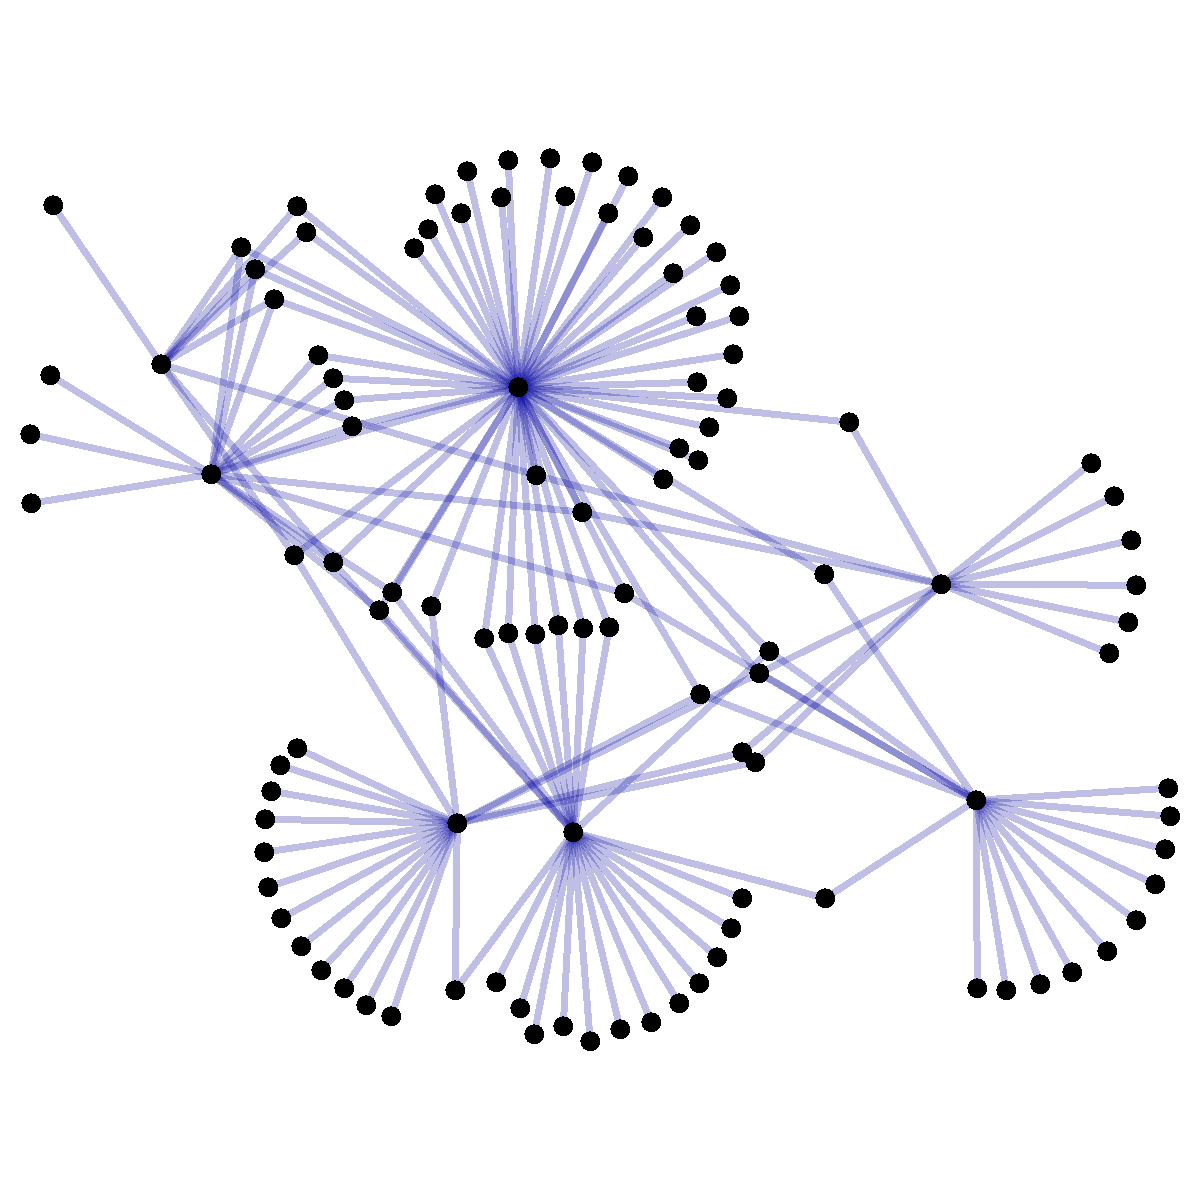
\includegraphics[width=\linewidth]{simple_graph.png}
\vspace*{-10mm}
\caption{A small example of a \textsl{connected} \textsl{simple} graph (\textsl{undirected} and \textsl{anti-reflexive}).}
\label{fig:simple_graph}
\end{wrapfigure}


\autoref{fig:simple_graph} is an illustration of a connected simple graph with 110 nodes and 151 edges.
I used graphs like this for testing purposes when developing \graffs.

\begin{definition}[Relations on graphs]
    \begin{itemize}[leftmargin=*]
        \item $G' = (V', E')$ is a \textbf{subgraph} of $G = (V, E)$ iff $V' \subseteq V$ and $E' \subseteq E$
        \item Let $G_1 = (V_1, E_1)$ and $G_2 = (v_2, E_2)$, then $G_1 \cup G_2 = (V_1 \cup V_2, E_1 \cup E_2)$ is the \textbf{union} of the two graphs, and $G_1 \cap G_2 = (V_1 {\cap} V_2, E_1 {\cap} E_2)$ is the \textbf{intersection} of the two graphs.
    \end{itemize}
\end{definition}

\begin{definition}[Node adjacency]
    \begin{itemize}[leftmargin=*]
        \item In an undirected graph, $v_1$ is \textbf{adjacent} to $v_2$ iff $(v_1, v_2) \in E$
        \item A \textbf{loop} is an edge of the form $(v, v)$.
        Note that simple graphs have no loops.
        \item Define $\deg^-(v) = \left| \Set{v' \in V}{(v', v) \in E} \right|$ to be the \textbf{indegree} of $v$, and $\deg^+(v) = \left| \Set{v' \in V}{(v, v') \in E} \right|$ to be the \textbf{outdegree} of $v$, in other words, the number of incoming and outcoming edges, respectively.
        If the graph is undirected, then $\deg^-(v) = \deg^+(v) = \deg(v)$ is called \textbf{degree}.
        \item For $G = (V, E)$ with $V = {1, 2, \dots, n}$, define $A = (a_{ij})$ to be the \textbf{adjacency matrix} of $G$ where
        \[ a_{ij} = \begin{cases}
                        1, & \textnormal{if}\ (i, j) \in E \\
                        0, & \textnormal{if}\ (i, j) \notin E
        \end{cases} \]
        for $1 \leq i, j \leq n$.

        Note that adjacency matrix of undirected graph is symmetric.
    \end{itemize}
\end{definition}

\begin{definition}[Connectedness]
    \begin{itemize}[leftmargin=*]
        \item $u, v$ are \textbf{connected nodes} is there exists a path between $u, v$ in $G$, i.e. if $(A^k)_{uv} = 1$ for some $k\in \mathbb{N}$.
        \item $G = (V, E)$ is \textbf{connected graph} if $\forall v_1, v_2 \in V. v_1, v_2$ are connected nodes.
        \item A subgraph $G' \subseteq G$ is a \textbf{(connected) component} iff $G'$ is a maximal connected subgraph of $G$.

        Note that all components of a graph are disjoint, therefore each node belongs to exactly one component.
    \end{itemize}

        \item A \textbf{giant component} of a graph is a single component that has more nodes than any other component of the graph.

        Note that a giant component may not exist, if more components have maximum number of nodes.
\end{definition}

\begin{figure}
\vspace*{-4mm}
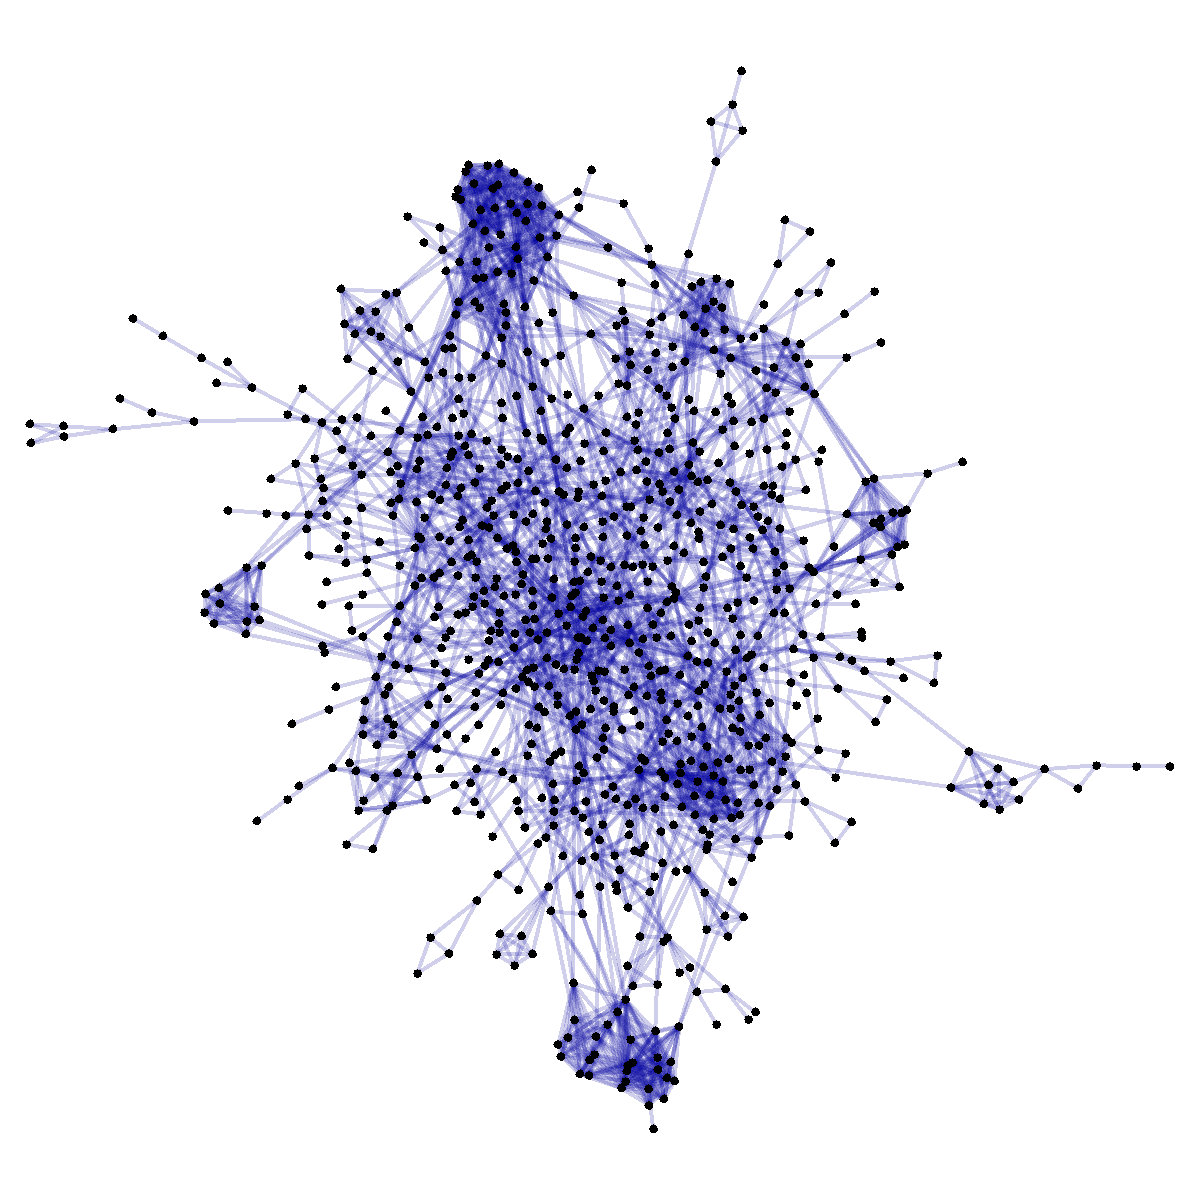
\includegraphics[height=6cm]{disconnecting_graph.png}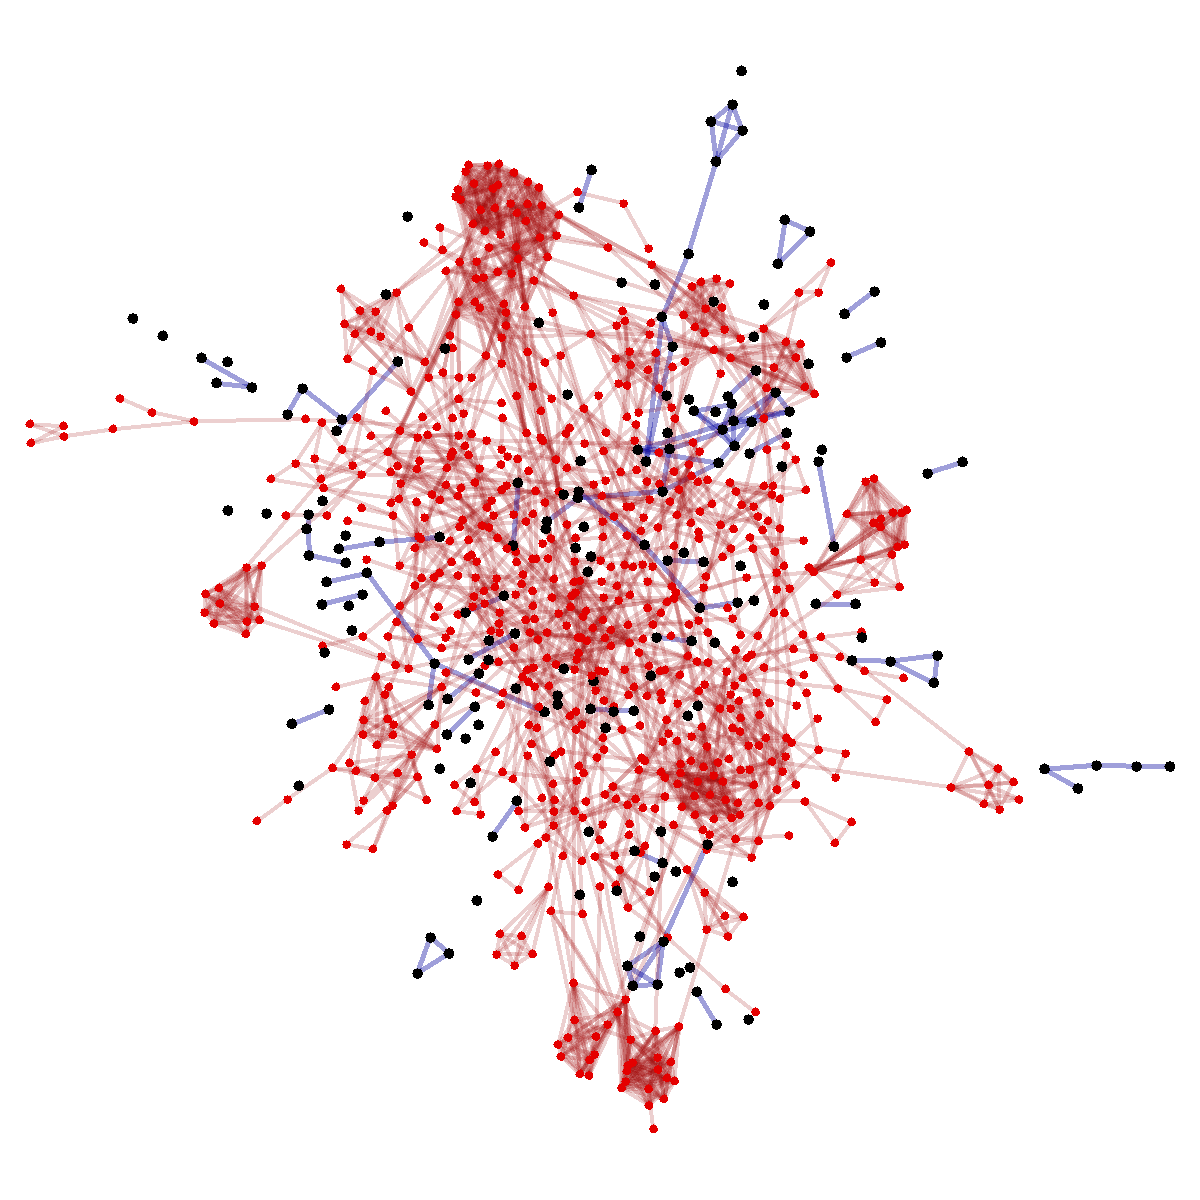
\includegraphics[height=6cm]{disconnecting_graph2.png}
\vspace*{-4mm}
\caption{Illustrated is how thresholding (a subgraph of) a protein network (left) results in one giant component (red) and multiple small disconnected components.
The left is a certain subgraph of the \textit{ecoli} dataset (all edges with confidence $>0.4$), the right graph has only edges with confidence $>0.5$.}
\label{fig:disconnecting_graph}
\end{figure}


Most of real-world networks (such as social networks, citation networks and even protein interaction networks) contain a single giant component, and some small isolated components.
For example, in \autoref{fig:disconnecting_graph}, the red nodes form a giant component of the graph.


\subsubsection{Networks}

Moving towards real-world data, graphs often emerge from a certain source in the world.
Just a few examples of the data possibly represented by graphs include social networks, road networks, computer networks, protein interaction networks, citation networks, web networks and so on.
In this work I distinguish graphs and networks, although I may sometimes interchange these two.

\begin{definition}[Network]
    A \textbf{network} is a graph whose nodes or edges can have attributes $\textnormal{attr}_v, \textnormal{attr}_e : \Sigma^* \rightarrow \mathbb{U}$ for some set of possible identifiers $\Sigma^*$ (such as a language over an alphabet $\Sigma$) and a value domain $\mathbb{U}$ (such as $\mathbb{R}$ or $\mathbb{R}^2$)
\end{definition}

Graphs and networks allow capturing the same structure, however, the main difference is that nodes of a network are \textit{identifiable}, while we rarely consider \textit{identity} of graph nodes.
%This is because nodes and edges of graphs coming from real-world are often (nearly) isomorphic to real-world objects and relations between them.
There may be either an exact or inexact matching between nodes/edges in the graph and objects/relations in the real world where the data came from (depending on whether the dataset is an approximation of the world).
I will often use networks when describing knowledge of the world.

\begin{definition}[Graph matching]
    Given two graphs $G = (V, E)$ and $G' = (V', E')$ derived from the same network, define \textbf{graph matching}, $M$, to be a bijection $V \leftrightarrow V'$ such that $(v, v') \in M$ iff $v, v'$ correspond to, or come from the same node in the network.
\end{definition}

For measuring metric robustness it will be beneficial to know matching between multiple graphs coming from the same dataset, or in other words to preserve identity of nodes across such graphs.

\subsection{Ranking}

\begin{definition}[Preorder]

\end{definition}

\begin{definition}[Total preorder]

\end{definition}

\subsection{Graph metrics}

Metrics are essentially functions of graphs that assign a value to each node.
Metrics allow quantifying various properties of graphs, identifying important nodes in different contexts, describing graph structures, comparing different graphs and more.
I study graph metrics as they are prominent and becoming even more crucial in analysing graphs of ever-growing real-world data.
With the increasing scale of emerging network datasets, it is becoming less possible to comprehend network structures just by visualisations.
Hence metrics are used to quantify properties of networks or their nodes.

In this chapter I describe the metrics that seem to be most significant for analysing protein interaction networks, and other graphs used in this project. The set of these metrics and their specific definition is based on The Paper\cite{Bozhilova2019}.

\subsubsection{Degree centrality}

One of the simplest metrics, degree centrality, calculates the degree of each node.

\begin{definition}
    For a graph $G = (V, E)$, define \textbf{degree centrality} $DC : V \rightarrow \mathbb{N}$ to be
    \[ DC(v) \eqdef \deg(v) = \left| \Set{v' \in V}{(v', v) \in E} \right| \]
\end{definition}

\subsubsection{Closeness centrality}

Closeness centrality of a node $v$ is the reciprocal value of the sum of $d(v, i)$, the distances from that node to all other nodes $i$ in the graph.

\[CC(v) = \frac{1}{\sum_{i \neq v} d(v, i)}\]

This is well defined for connected graphs, however, $d(v, i)$ is undefined if $v, i$ belong to two different components of the graph. For disconnected graphs, I set $d(v, i) = |V|$ to follow the approach in~\cite{Bozhilova2019}.

Closeness centrality measures, for each node, its reciprocal of the \textsl{farness} of the node to other nodes. Nodes with higher closeness centrality are \textsl{closer} to all other nodes.

A common alternative for disconnected graphs is to compute Harmonic centrality.

\subsubsection{Harmonic centrality}

Has similar meaning to closeness centrality, and a similar definition.

\[HC(v) = \sum_{i \neq v} \frac{1}{d(v, i)}\]
with $1 / d(v, i) = 0$ for disconnected nodes $v, i$.

\subsubsection{Eigenvector centrality}

\subsubsection{Katz centrality}
- not used much recently

\subsubsection{PageRank}
= Katz centrality, but divide each vertex's contribution by its out-degree

\subsubsection{Hyperlink-induced topic search (HITS)}
Hubs and authorities, by Kleinberg

% from GraphStream

\subsubsection{CommunityMeasure}
- Modularity\\
- Community Distribution\\
- CommunityRelativeMeasure $\rightarrow$ NormalizedMutualInformation $\rightarrow$ VariationOfInformation

\subsubsection{Eccentricity}

\subsubsection{Surprise measure}

\subsubsection{Degree measure}

\subsection{Robustness (The Paper)}

\subsection{Datasets}

Although the framework built is universal and is not bound to any datasets, I chose a number of datasets for evaluation.

\subsubsection{Stanford Large Network Dataset Collection}

The \textit{Stanford Large Network Dataset Collection}\cite{Large2016} provides open datasets obtained from real-world data such as social networks, citation networks, web graphs, internet networks, road networks and many more.

\subsubsection{STRING database}

\textit{STRING}\cite{Szklarczyk2019} is an open database of interactions between proteins.
At the time of writing, the database contains over 24M different proteins from over 5K organisms.

Considering the whole graph as an input for this project would be unsuitable because of its size, but for the evaluation, sub-graphs of proteins of only certain organisms will be used.

Note that, generally, one cannot just consider a sub-graph of a source graph (such as sub-graph of a social network), because the generated sub-graph doesn't have a semantic meaning, and its characteristic heavily depend on how the graph was generated (for example, $n$ friends of one person would result in a more connected graph than $n$ random people in the world).
However, sub-graphs of the STRING database built from proteins of concrete organism can be used, because such graphs alone have a semantic meaning.

\subsubsection{KONECT}

KONECT - The koblenz network collection\cite{Kunegis2013}

\subsubsection{Generating graphs}

Possible algorithms to use: \url{https://jgrapht.org/javadoc/org/jgrapht/generate/package-summary.html}


\section{Methods}

In particular, this chapter will discuss mainly the following, in the theoretical framework:
\begin{itemize}
    \item collecting source datasets
    \item generating distorted graphs
    \item common graph metrics that can evaluated on graphs
    \item ways to quantify robustness of metrics
\end{itemize}



    \chapter{Implementation}\label{ch:implementation}
    This chapter describes first the overall structure of the project, its technical requirements (which can and later be used as part of the evaluation) and then dives into the implementation of individual modules.

I refer to this project by its name \textsl{graffs}.
A working version is published on GitHub\footnote{\url{https://github.com/jjurm/graffs}} along with its source code.


\section{Overview}

The purpose of this project is to develop a methodology and tool, i.e. a framework, to help study graph metrics, and empirically analyse their robustness in particular.

\graffs is a command-line tool written in Kotlin that can load/store datasets of different formats, generate perturbed graphs, evaluate metrics, and calculate robustness values. \autoref{fig:brief_pipeline} is a diagram explaining the natural flow of the program, i.e. the \textsl{main pipeline} starting with graph datasets and ending up with deductions about each metric's \textsl{robustness}.

\begin{figure}[ht]
    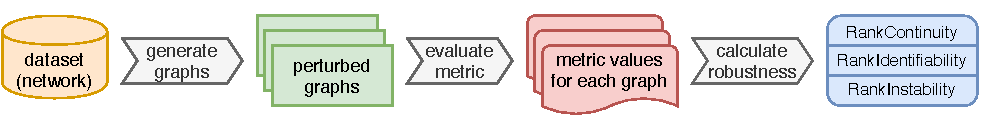
\includegraphics[width=\linewidth]{brief_pipeline.pdf}
    \caption{A brief illustration of the evaluation process.
    A generator is used to generate perturbed graphs from an input dataset.
    A chosen metric is evaluated on all petrurbed graphs, producing per-node values.
    Finally, each robustness measure's value of the metric is calculated.
    This is referred to as the ``Main pipeline'', explained further in \cref{fig:main_data_flow}.}
    \label{fig:brief_pipeline}
\end{figure}


\section{Design goals}\label{sec:design-goals}

The following are technical requirements I set for the project.
Overall, I aim this tool to be reusable for similar projects, either by directly invoking the compiled binary, or by using it as a dependency, or by forking and extending it.
The target user is a researcher or anyone who would benefit from assessing the stability of graph metrics evaluated on arbitrary graphs.

\subsection{Supported features}

\graffs supports the following features:

\begin{enumerate}[itemsep=0pt,topsep=5pt]
    \item Store, load input graphs in various formats, and represent them in a unified memory structure
    \item Run algorithms that compute metrics on graphs
    \item Generate graphs by applying perturbations to given input graphs
    \item Run experiments by evaluating metrics on generated graphs in a systematic manner
    \item Calculate robustness of metrics based on experiments
    \item Possibly, produce visual output from the results
\end{enumerate}

\subsection{Scalability}

According to The Paper~\cite{Bozhilova2019}, calculating natural connectivity for a single node for a graph with ~7000 nodes takes ~88 seconds on a standard computer.
In one of my toy examples, calculating average betweenness centrality of ~2500 nodes took ~8 minutes on my personal computer.
Thus, assuming computing a (computation-heavy) metric(s) on an input graph of average size 5000 nodes takes ~30 minutes, the pure computation time suggested by the~\nameref{ch:proposal} would take the following time on a standard personal computer (approximated in the order of magnitude)
\[(\sim 6\ \text{datasets}) \times (\sim 6\ \text{metrics}) \times (\sim 50\ \text{derived graphs}) \times (\sim 30\ \text{minutes}) \approx 38\ \text{days}\]

For this reason, one of the goals is to make the program efficient and runnable on a supercomputer, utilising the power of high-performance \textbf{multi-core systems} for \textbf{parallel execution}.

\subsection{Reproducibility}\label{sec:reproducibility}

It is important for all results in research to be reproducible.
By \textsl{reproducibility} of \graffs I mean the guarantee that one can exactly reproduce any results produced by the program.
I.e. when the program is run two times with the same input and hyper-parameters, it must produce the same output.
And by \textsl{the same output} I mean producing the same robustness results, images, tables, numbers up to a bit-wise match where applicable.

This is a challenge in all the following areas:
\begin{itemize}
    \item \textbf{Stochastic processes}

    Methods based on stochastic processes or randomness must be reproducible.
    An example of a stochastic method are graph generators.

    These can be made reproducible done by generating all randomness starting off with a given seed for the generator.

    \item \textbf{Resolving ties}

    Methods that are not inherently stochastic but require pseudo-randomness to resolve ties must also be reproducible.
    An example is ranking nodes of a graph according to metric values, or generating a visual layout for graphs such as in \autoref{fig:simple_graph}.

    Again, a solution is to base such flow on an input seed.

    \item \textbf{External factors}

    Unpredictability introduced by the operating system and other external factors must be accounted for, so that the program still produces the same results even if run on a different supported machine, in a different environment.
    This is more challenging in a concurrent environment when it must be made sure the produced output does not depend on any factors such as uncertainty and unpredictability of the OS's thread scheduler.

    These issues are resolved using a robust programming language and concurrency synchronisation approaches.
\end{itemize}

\subsection{Flexibility}

The program must be flexible enough, in particular the following:
\begin{enumerate}
    \item Usable on all widely used machines and operating systems
    \item Accepting input datasets (and any input parameters) in common formats
    \item As a library, it must provide modular access to individual parts of the program, so that it is easy to use \graffs as a dependency in future projects of a similar kind
\end{enumerate}


\section{Architecture}

In this section I explain major decisions about the program, such as the choice of the Kotlin language, and Git, Gradle tools.

\subsection{Kotlin language}

I used the programming language \textbf{Kotlin}, mainly for the following reasons.
It is by nature similar to Java and can be used together with other Java code in a single project.
Performance-wise, Kotlin is comparable to Java.
\begin{itemize}
    \item Concise, reducing the amount of boilerplate code
    \item Safer, preventing a significant number of errors
    \item IDE-friendly, allowing the IDE to help with software engineering
    \item Employs functional programming paradigms~\cite{Bonev}
    \item Compiles to Java byte code and so preserves other important benefits of Java: Object-Oriented, multi-threaded, platform-independent, secure and easily extensible.
\end{itemize}

Using Kotlin in the project still allows including any libraries written in Java, as Kotlin compiler compiles \texttt{.kt} files to Java-bytecode \texttt{.class} files.
Kotlin has most of its concepts and features adopted from Java, such as classes, polymorphism, inheritance, so these concepts I will freely use in this work.

Kotlin has a number of advanced features such as improved type safety and reduced boilerplate code~\cite{JemerovKotlinAction2017}.
There is one notable feature of Kotlin: properties.
Properties are an abstraction of fields and getters/setters in classes and help decouple the implementation of the class from its interface even more.
In UML diagrams in this work , instead of presenting fields and methods of each class, listed are methods and properties (in this order).

\subsection{Version Control System}

The source code of the \graffs tool is stored in a Git repository, which keeps track of all code changes and allows understanding how code changed over time as well as restoring previous versions.

The repository can be found at \url{https://github.com/jjurm/graffs}.

\subsection{Build automation}

The project uses Gradle~\cite{BerglundBuildingTestingGradle2011} for project management.
Split into different modules, Gradle also helps to keep the structure well defined and manages builds of each module separately (which is called a multi-project build in Gradle).

Project configuration rules are set up using the \texttt{build.gradle} files (one in the root directory, then one within each module) with a number of plugins to facilitate the following and more:
\begin{enumerate}
    \item Defines the structure of the project, such as the directories for each module, and source and build directories of each
    \item Automates the process of compiling the code, running tests and producing deployable \texttt{jar}s
    \item Manages and automatically downloads dependencies
    \item Helps with version numbering
    \item Generates HTML API documentation for Kotlin code documented using the \texttt{KDoc} language\footnote{Using the \texttt{Dokka} tool, similar to \texttt{JavaDoc}}
\end{enumerate}

\subsection{Computing cluster}\label{sec:computing_cluster}

I used a remote high-performance computing facility provided by the Systems Research Group (\url{https://www.cl.cam.ac.uk/research/srg/}), sponsored by Dr Andrew Moore (\url{andrew.moore@cl.cam.ac.uk}).

In particular, I worked with the following servers:

\begin{description}
    \item[\texttt{rio.cl.cam.ac.uk}] server running \textsl{Ubuntu 18}, using \textsl{4x 8-Core AMD Opteron 6128} with 16 MiB L2 cache (32 cores in total), and 128 GiB RAM
    \item[\texttt{nile.cl.cam.ac.uk}] server running \textsl{Ubuntu 18}, using \textsl{2x 12-Core AMD Opteron 6168} with 12 MiB L2 cache (24 cores in total), and 128 GiB RAM
\end{description}

The \graffs tool is programmed in a way which utilizes many threads to allow parallel computing.
There are a number of frameworks that can aid in high-performance computing, and I analysed a few.
I installed and experimented with Apache Spark~\cite{ZahariaApacheSparkUnified2016}, and investigated a number of other off-the-shelf products such as Apache Storm and Spring Boot -- although these libraries support computation across multiple machines, they are more heavyweight.
To make \graffs portable as part of the flexibility goal, I opted in for a solution that does not require installing or setting up such framework for running the tool, in particular the \texttt{kotlinx.coroutines} library~\cite{TorresLearningConcurrencyKotlin2018} (see~\autoref{sec:kotlin_coroutines}), with the small tradeoff that this does not allow distributed computing across multiple machines out of the box.

\subsubsection*{Setting up the cluster}

\subsection{Project modules}

The project is structured in the following modules, using multi-project builds in Gradle:
\begin{itemize}
    \item \texttt{core} - APIs for structures, metrics, generators, etc., as well as the core data model for storing data in the database
    \item \texttt{storage} - accessing and loading graphs/datasets stored in the filesystem
    \item \texttt{generators} - graph generators
    \item \texttt{metrics} - graph metrics
    \item \texttt{robustness} - robustness measures
    \item \texttt{cli} - code for command-line interface
\end{itemize}


\section{Data model}

The \graffs tool uses a number of libraries to represent graphs in memory, define a data model, and store data in a relational database.
This section explains how the data of the program is persisted.

The following entities highligh the main concept, and there are some more entities stored in the database.
\begin{itemize}[topsep=5pt]
    \item \textsl{Graph} storing its nodes, edges (and their attributes)
    \item \textsl{Graph generator} is an object capable of producing a number of graphs, given a dataset.
    \item \textsl{Experiment} is a description of a computational task involving:
    \begin{enumerate}[topsep=5pt]
        \item generating graphs from given input datasets using a given graph generator
        \item evaluating a given set of metrics on all generated graphs
        \item evaluate given robustness measures on all metrics over all datasets of the experiment
    \end{enumerate}
\end{itemize}

A user can create and manage \textsl{graph generators} and \textsl{experiments} using the command line interface (see \autoref{sec:cli}).

\subsection{Using GraphStream}\label{sec:graphstream}

Graphs in memory are stored and manipulated by the GraphStream library~\cite{DutotGraphStreamToolBridging2007}, a \enquote{Java library for the modeling and analysis of dynamic graphs. You can generate, import, export, measure, layout and visualize them}.\footnote{As alternatives, I also investigated and considered library JGraphT~\cite{Michail2019}, which is algorithm-focused, however, the algorithms relate mostly to walking on graph nodes and are not relevant for evaluating graph metrics.
GraphStream also provides visualisations as opposed to JGraphT.}
The library consists of 3 modules: \texttt{gs-core} defining the API and underlying structures, \texttt{gs-algo} with various algorithms from graph theory, and \texttt{gs-ui} containing components for visualising graphs.

\begin{figure}[ht]
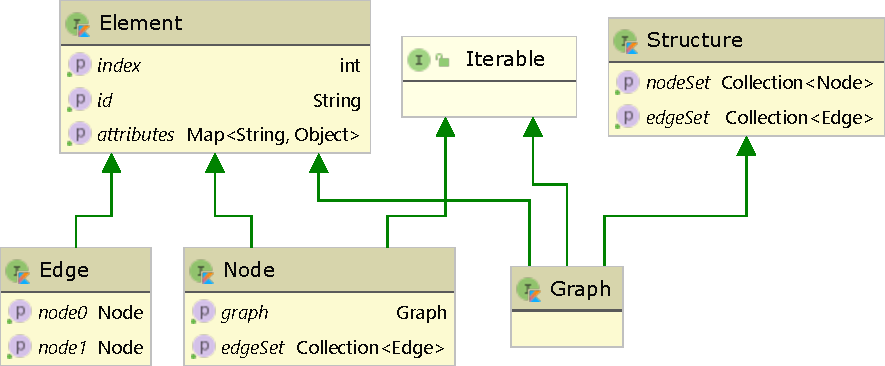
\includegraphics[width=0.65\linewidth]{graphstream_diagram.pdf}
\caption{A simplified diagram of key interfaces from the GraphStream library}
\label{fig:graphstream_diagram}
\end{figure}


The library is based around the \texttt{Graph} interface, which provides access to \texttt{Node}s and \texttt{Edge}s of each graph.
The most relevant interfaces are illustrated in \autoref{fig:graphstream_diagram} (heavily simplified).
The interfaces also provide methods for changing graphs (adding/removing nodes, edges, attributes, etc.).
In practice the library's interfaces contain many more links and methods (e.g. for handling directed graphs) that are not relevant in the context of this project.

For evaluation of robustness, we need to be able to compare (ranks of) values of a specific node between two or more generated graphs, therefore we need to be able to preserve mapping of nodes of a generated graph to nodes in the original dataset (see \autoref{def:graph_matching}).
Note that all \texttt{Element}s (i.e. \texttt{Node}s, \texttt{Edge}s and even \texttt{Graph}s) have an \texttt{id} field which will be used for matching nodes between base and perturbed graphs.
This makes evaluation of robustness more straightforward as ranks of nodes in respect to a given metric can be compared across multiple graphs generated from the same base graph.

The GraphStream library also provides a solid base for numerous features in this project such as loading graph files, storing them in various formats, and visualisations.
The GraphStream library allows working with dynamic graphs (changing over time), my project only uses static graphs.
The library also contains an implementation of some graph metrics.

\parspace

The \texttt{Graph} object from the GraphStream library stores (references) all nodes and edges, along with attributes.
In my project, if a metric has been evaluated on a graph, the metric's value for each node is stored as the \texttt{Node}'s attribute, all contained within the \texttt{Graph} object.
The attribute key is given my the metric name.

\subsection{Relational model}

Data of the \graffs tool such as generated graphs, evaluated metrics, robustness measure results as well as any user-defined hyper-parameters are stored in a relational database system.
The Java Persistence API (JPA)~\cite{BiswasJavaPersistenceAPI2016} provides an abstraction for accessing relational data from Java, Hibernate~\cite{ElliottHibernateDeveloperNotebook2004,BauerJavaPersistenceHibernate2015} is a framework that implements the inteface.
I used specifically the H2 database engine~\cite{MuellerH2DatabaseEngine2006} as the underlying storage for Hibernate.
This abstraction is later illustrated in \autoref{fig:orm_kotlin_h2_diagram}.

\begin{figure}
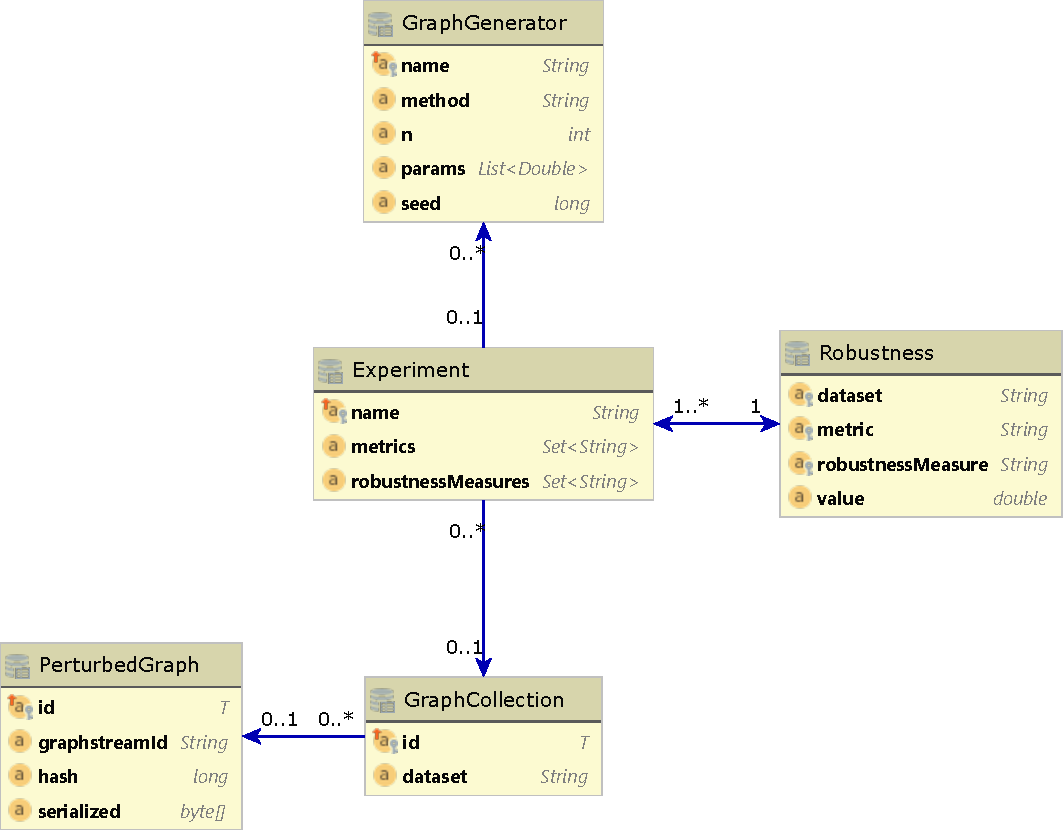
\includegraphics[width=0.9\linewidth]{data_model_diagram.pdf}
\caption{Data model diagram showing \textsl{persistence schema}, i.e. entities stored in the database.
The arrows indicate \textsl{association} links, i.e. ``has a'' or ``refers to'' relationships.
The diagram is created from the Java Persistence API schema inferred from the source code.}
\label{fig:data_model_diagram}
\end{figure}


\autoref{fig:data_model_diagram} shows the entities that the program persists in the database, as explained below.
Named entities (\texttt{Experiment}, \texttt{GraphGenerator}) are those that the user creates and later refers to with their name.
\begin{description}[itemsep=\zerospace]
    \item[\texttt{PerturbedGraph}]
    stores a serialised version of the \texttt{Graph} object, inclucing all so-far evaluated metric values of nodes, and possibly a weight associated with each edge (for scored networks).
    It also stores metadata, such as a hash which distinguishes the graph from other graphs beloging to the same \texttt{GraphCollection} coming from the same graph generator.
    For example in the case graphs are generated by \hyperref[sec:randomly_removing_edges]{randomly removing edges}, the starting seed value of the generator of the particular graph is used as its hash.

    \item[\texttt{GraphCollection}]
    represents an (ordered) collection of \texttt{PerturbedGraph}s.
    It also keeps track of which datasets the graphs were generated from.

    \item[\texttt{GraphGenerator}]
    is an entity that stores user-defined rules for generating graphs from a dataset.
    Once a graph generator is defined and created, it can universally be used on multiple input datasets.
    The parameters of a generator include the name of the method to use (such as \texttt{linear-thresholding}), number of perturbed graphs to generate from each input dataset, seed, and any additional numeric parameters specific to each generator.

    \item[\texttt{Experiment}]
    an entity that encapsulates a concept of evaluating multiple \textsl{robustness measures} of multiple \textsl{metrics} on multiple \textsl{datasets}, using a specific graph generator.
    With an existing generator, the user defines an experiment, which can then be evaluated (see \autoref{sec:main_pipeline}).

    \item[\texttt{Robustness}]
    an entity that stores a single result of evaluating a \textsl{robustness measure} of a \textsl{metric}, on a set of perturbed graphs originating from a certain \textsl{dataset}.
    These robustness values each belong to its parent \texttt{Experiment}.
    Note (\autoref{fig:data_model_diagram}) that the four fields \texttt{experiment}, \texttt{dataset}, \texttt{metric}, \texttt{robustnessMeasure} together form the primary key.
\end{description}

\subsection{Java Persistence API}

The Java Persistence API~\cite{BiswasJavaPersistenceAPI2016} (JPA) is an API specification for management of relational data in Java.
It describes ways in Java to specify schemas of relational databases and an interface to manage and access data of a relational model (i.e. entities in tables, relations, first-order logic).
\textsl{Persistence} is an abstract term referring to accessing, managing, and storing entities.

The Hibernate framework~\cite{ElliottHibernateDeveloperNotebook2004}, an object-relational mapping tool, provides a concrete implementation of JPA~\cite{BauerJavaPersistenceHibernate2015}.
I use Hibernate as the intermediate layer between the \texttt{core} module of \graffs and the underlying H2 database that is completely abstracted away from the \graffs code (\autoref{fig:orm_kotlin_h2_diagram}).

\begin{figure}[ht]
    \vspace*{0.3cm}

    \tikzset{every picture/.style={line width=0.75pt}} %set default line width to 0.75pt

    \begin{tikzpicture}[x=0.75pt,y=0.75pt,yscale=-1,xscale=1]
%uncomment if require: \path (0,182); %set diagram left start at 0, and has height of 182

%Flowchart: Document [id:dp21196524185892507]
        \draw  [fill={rgb, 255:red, 215; green, 213; blue, 186 }  ,fill opacity=1 ][line width=1.5] [blur shadow={shadow xshift=2.25pt,shadow yshift=-1.5pt, shadow blur radius=1.5pt, shadow blur steps=4 ,shadow opacity=45}] (27.93,54) -- (130,54) -- (130,115.84) .. controls (66.2,115.84) and (78.96,138.14) .. (27.93,123.71) -- cycle ;
%Image [id:dp8157383933237885]
        \draw (76.96,73.21) node  {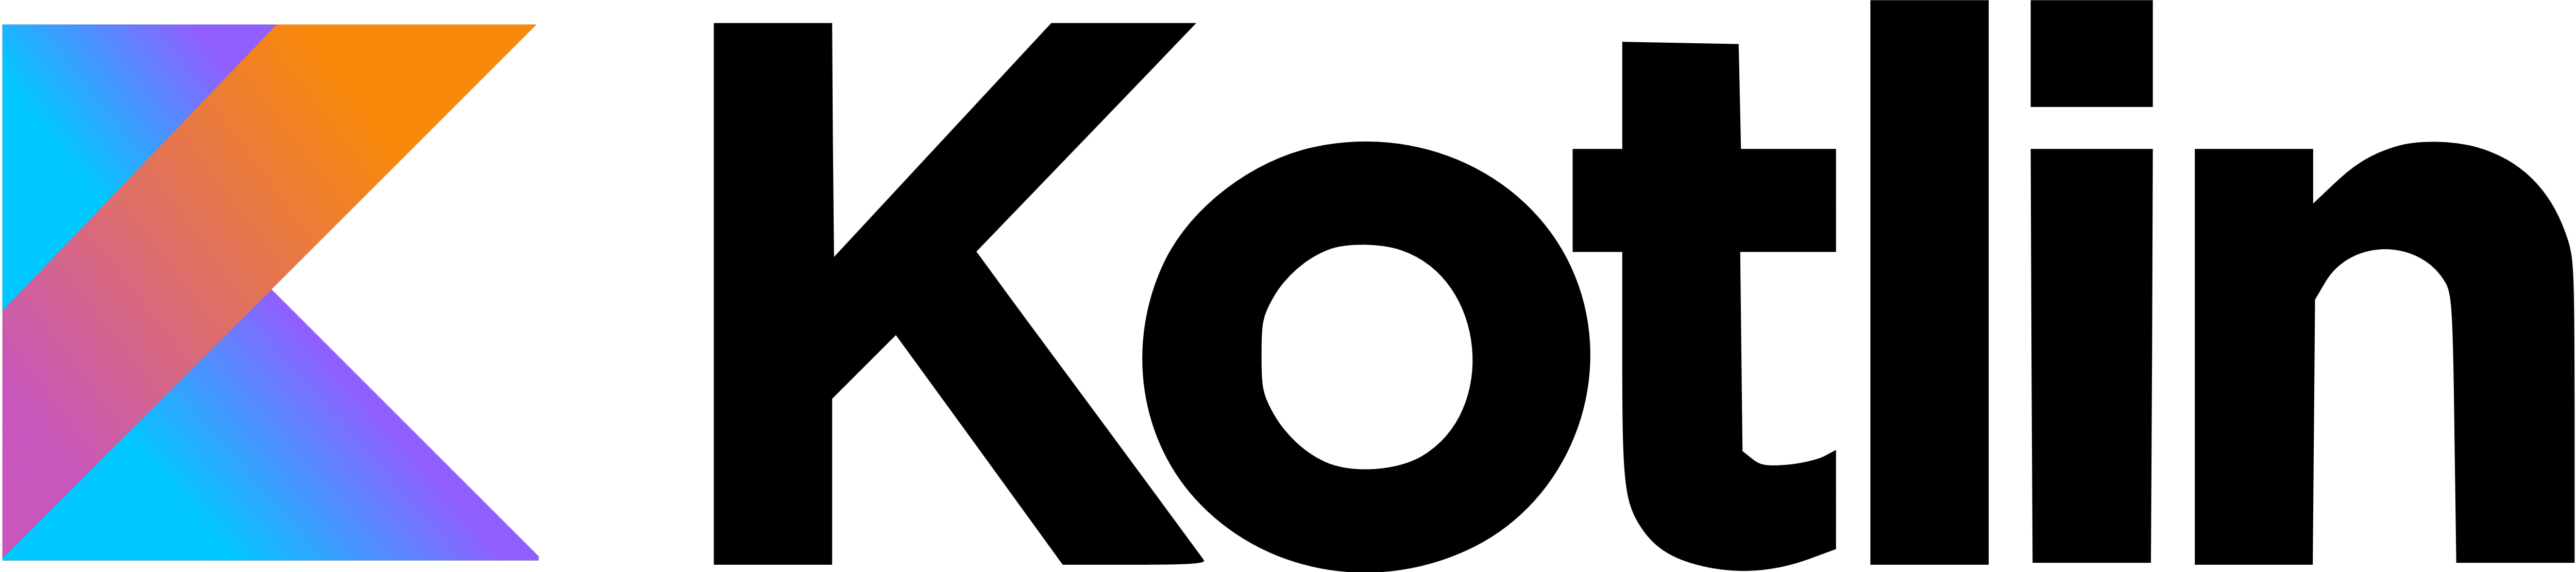
\includegraphics[width=55.44pt,height=12.32pt]{Kotlin_logo_wordmark.png}};
%Shape: Diamond [id:dp1258210345503794]
        \draw  [fill={rgb, 255:red, 247; green, 244; blue, 209 }  ,fill opacity=1 ][line width=1.5] [blur shadow={shadow xshift=2.25pt,shadow yshift=-1.5pt, shadow blur radius=1.5pt, shadow blur steps=4 ,shadow opacity=45}] (314,54.96) -- (368.93,93.75) -- (314,132.54) -- (259.07,93.75) -- cycle ;
%Image [id:dp807711922850731]
        \draw (312.63,92.23) node  {
\includegraphics[width=71.69pt,height=19.9pt]{Hibernate_logo_a.png}};
%Flowchart: Magnetic Disk [id:dp301549321862431]
        \draw  [fill={rgb, 255:red, 16; green, 33; blue, 255 }  ,fill opacity=1 ][line width=1.5] [blur shadow={shadow xshift=2.25pt,shadow yshift=-1.5pt, shadow blur radius=1.5pt, shadow blur steps=4 ,shadow opacity=45}] (522,72.08) -- (522,113.38) .. controls (522,119.52) and (505.45,124.5) .. (485.03,124.5) .. controls (464.61,124.5) and (448.06,119.52) .. (448.06,113.38) -- (448.06,72.08)(522,72.08) .. controls (522,78.22) and (505.45,83.2) .. (485.03,83.2) .. controls (464.61,83.2) and (448.06,78.22) .. (448.06,72.08) .. controls (448.06,65.94) and (464.61,60.96) .. (485.03,60.96) .. controls (505.45,60.96) and (522,65.94) .. (522,72.08) -- cycle ;
%Image [id:dp005669783415606533]
        \draw (496.46,97.63) node  {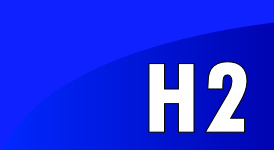
\includegraphics[width=36.81pt,height=20.15pt]{h2-logo.png}};
%Flowchart: Connector [id:dp7113910887207657]
        \draw  [color={rgb, 255:red, 0; green, 0; blue, 0 }  ,draw opacity=1 ][fill={rgb, 255:red, 86; green, 99; blue, 255 }  ,fill opacity=1 ][line width=1.5]  (448.06,72.08) .. controls (448.06,65.94) and (464.61,60.96) .. (485.03,60.96) .. controls (505.45,60.96) and (522,65.94) .. (522,72.08) .. controls (522,78.22) and (505.45,83.2) .. (485.03,83.2) .. controls (464.61,83.2) and (448.06,78.22) .. (448.06,72.08) -- cycle ;
%Straight Lines [id:da18726463966554463]
        \draw [line width=1.5]    (133.93,93.75) -- (255.93,93.75) ;
        \draw [shift={(258.93,93.75)}, rotate = 180] [color={rgb, 255:red, 0; green, 0; blue, 0 }  ][line width=1.5]    (14.21,-4.28) .. controls (9.04,-1.82) and (4.3,-0.39) .. (0,0) .. controls (4.3,0.39) and (9.04,1.82) .. (14.21,4.28)   ;
        \draw [shift={(130.93,93.75)}, rotate = 0] [color={rgb, 255:red, 0; green, 0; blue, 0 }  ][line width=1.5]    (14.21,-4.28) .. controls (9.04,-1.82) and (4.3,-0.39) .. (0,0) .. controls (4.3,0.39) and (9.04,1.82) .. (14.21,4.28)   ;
%Straight Lines [id:da6738825729018745]
        \draw [line width=1.5]    (371.93,93.75) -- (442.93,93.75) ;
        \draw [shift={(445.93,93.75)}, rotate = 180] [color={rgb, 255:red, 0; green, 0; blue, 0 }  ][line width=1.5]    (14.21,-4.28) .. controls (9.04,-1.82) and (4.3,-0.39) .. (0,0) .. controls (4.3,0.39) and (9.04,1.82) .. (14.21,4.28)   ;
        \draw [shift={(368.93,93.75)}, rotate = 0] [color={rgb, 255:red, 0; green, 0; blue, 0 }  ][line width=1.5]    (14.21,-4.28) .. controls (9.04,-1.82) and (4.3,-0.39) .. (0,0) .. controls (4.3,0.39) and (9.04,1.82) .. (14.21,4.28)   ;

% Text Node
        \draw (473,66) node [anchor=north west][inner sep=0.75pt]  [font=\small,color={rgb, 255:red, 255; green, 255; blue, 255 }  ,opacity=1 ,xslant=0.11] [align=left] {\textbf{DB}};
% Text Node
        \draw (59,86) node [anchor=north west][inner sep=0.75pt]  [font=\small,color={rgb, 255:red, 0; green, 0; blue, 0 }  ,opacity=0.8 ] [align=left] {code};
% Text Node
        \draw (295,103) node [anchor=north west][inner sep=0.75pt]  [font=\small,color={rgb, 255:red, 0; green, 0; blue, 0 }  ,opacity=0.8 ] [align=left] {ORM};
% Text Node
        \draw (140,53) node [anchor=north west][inner sep=0.75pt]  [font=\small] [align=left] {Java \\method invocation};
% Text Node
        \draw (390,72) node [anchor=north west][inner sep=0.75pt]   [align=left] {SQL};

    \end{tikzpicture}

    \caption{Diagram of Hibernate operating as a middle layer between Kotlin code and the underlying H2 database}
    \label{fig:orm_kotlin_h2_diagram}
\end{figure}


\begin{figure}
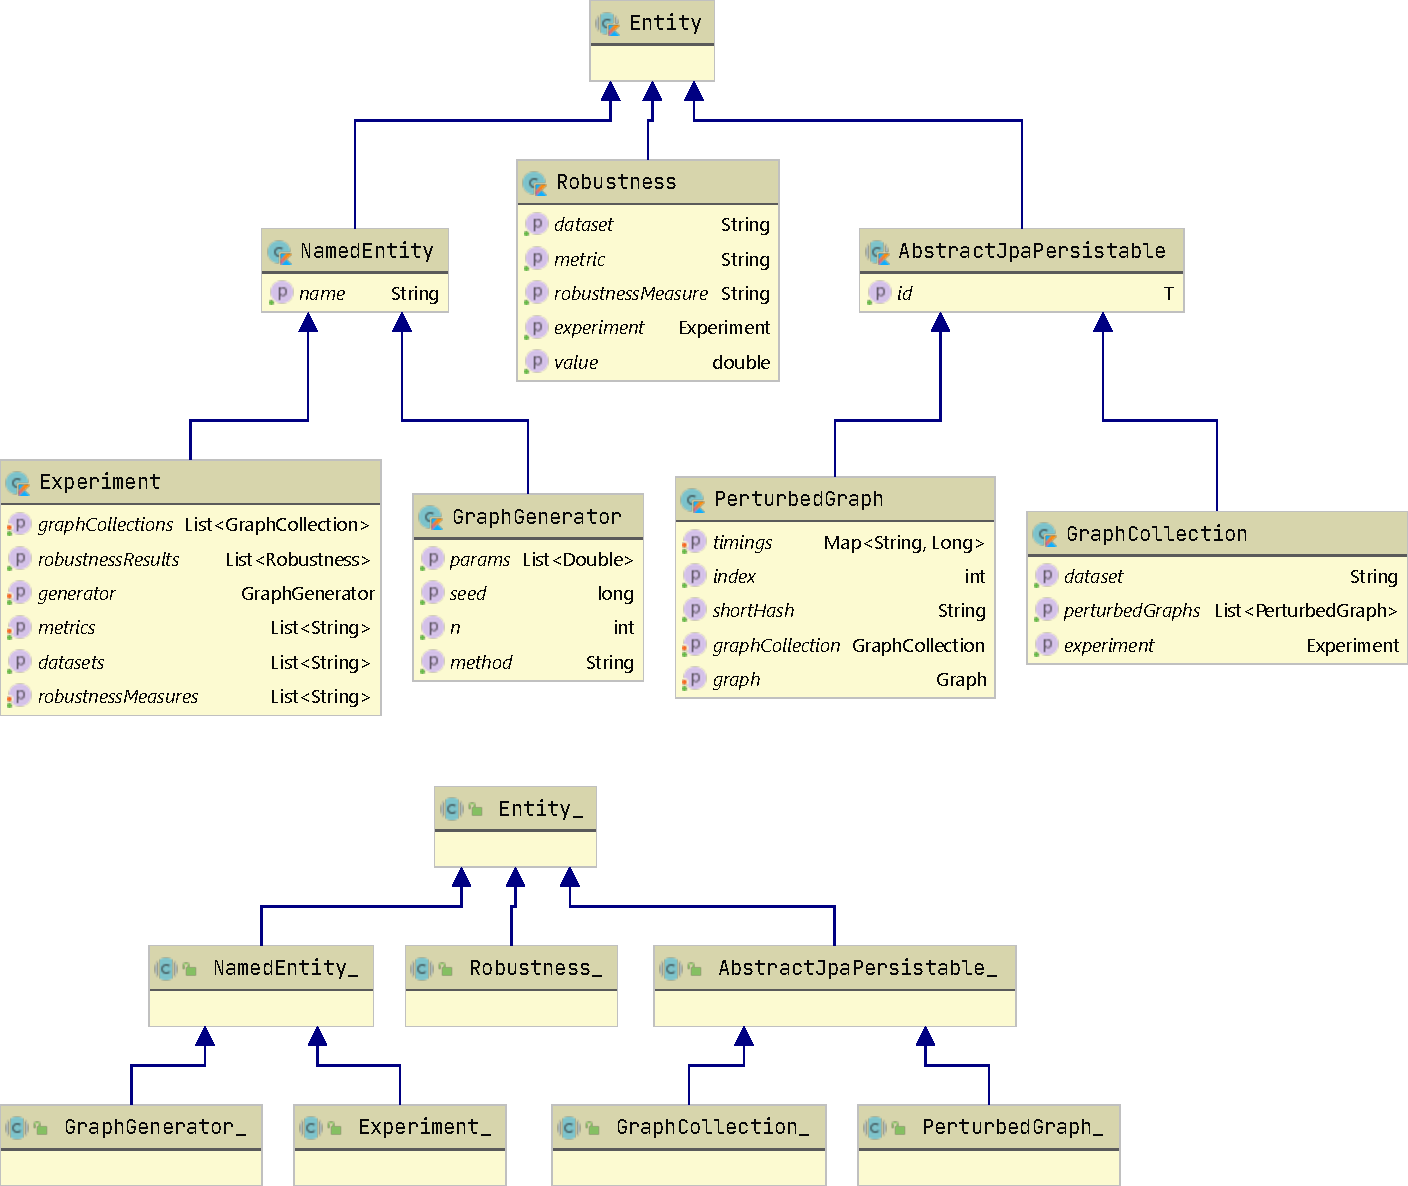
\includegraphics[width=\linewidth]{data_model_classes_diagram.pdf}
\caption{Inheritance hierarchy of the (Kotlin) classes underlying the persistence model presented in \autoref{fig:data_model_diagram}.
The arrows indicate \textsl{inheritance} (``is a'') relationships between classes.}
\label{fig:data_model_classes_diagram}
\end{figure}


Further, \autoref{fig:data_model_classes_diagram} shows the underlying \textsl{entity classes} written in Kotlin that have the following functions:
\begin{itemize}[topsep=5pt,label=$\bm{\rightarrow}$]
    \item \textbf{Data model definition}, seen in \autoref{fig:data_model_diagram}

    JPA provides a number of Java annotations to define entities (\texttt{@Entity}), their fields (\texttt{@Column}), constraints such as foreign key constraint (\texttt{@OneToMany}, \texttt{@ManyToOne} and others), and metadata such as rules for fetching data from database (e.g. \texttt{@Basic(fetch = FetchType.LAZY)} for lazy fetching of a field).
    Data model is inferred from these annotations that are processed during compile time

    Hibernate then abstracts away also operations such as creating and updating the database schema, which are configured in the \texttt{hibernate.cfg.xml} file (for example it creates a database from scratch if it doesn't exist).

    See \autoref{lst:kotlin_experiment_entity} for an example entity class using the JPA annotations.

    \item \textbf{Metamodel generation}

    Taking the annotated entity classes during compile time, Hibernate generates a \textsl{metamodel} class for each entity to allow writing type-safe queries.
    For example, the \texttt{Experiment\_} class is generated from the \texttt{Experiment} entity, with corresponding fields (such as \texttt{Experiment\_.name} of type \texttt{SingularAttribute<NamedEntity, String>}, or \texttt{Experiment\_.generator} of type \texttt{SingularAttribute<Experiment, GraphGenerator>}).

    See \autoref{lst:jpa_typed_query} for an illustration how generated metamodel classes aid in writing type-safe queries.

    \lstinputlisting[label={lst:jpa_typed_query}, linerange=jpa_typed_query0-jpa_typed_query1, caption={A toy example of using typed JPA queries. Note the \texttt{Experiment\_} metamodel class generated by Hibernate with (meta)fields corresponding to entities' fields}, float, language=Kotlin]{listings.kts}

    \item \textbf{Object-relational mapping}

    The classes (\autoref{fig:data_model_classes_diagram}) themselves carry the data managed by Hibernate.
    This means that other modules such as \texttt{generators} and \texttt{robustness} can use entity classes, while they are also managed by Hibernate.

    Hibernate is responsible for loading data into entity objects as well as persisting such objects.
    See \autoref{lst:hibernate_load_entity} for an illustration.

    \lstinputlisting[label={lst:hibernate_load_entity}, linerange=hibernate_load_entity0-hibernate_load_entity1, caption={A toy example of Hibernate loading and persisting an \texttt{Experiment} object.}, float, language=Kotlin]{listings.kts}
\end{itemize}


\autoref{lst:kotlin_experiment_entity} presents a full code listing of the \texttt{Experiment} entity.

\lstinputlisting[label={lst:kotlin_experiment_entity}, caption={The \texttt{Experiment} class written in Kotlin. Note especially the annotations which are enough to define the JPA data model.}, float, firstline=11,language=Kotlin]{Experiment.kt}

\subsection{H2 Database}

I employed the H2 relational database~\cite{MuellerH2DatabaseEngine2006} (based on SQL language) for storing entities, considering the following:
\begin{itemize}[topsep=5pt]
    \item Very fast; small footprint on the system in terms of installation complexity, program size, and cost of backround maintenance
    \item Easily embeddable, as it implements the JDBC API (Java Database Connectivity API, used by Hibernate too)
    \item Supports in-memory databases (good for testing)
    \item Written purely in Java, so can be bundled in \graffs and thus requires no other database installation in the client OS
\end{itemize}

\subsubsection*{Storing graphs in database}

Considering exporting graphs to various formats, I chose to store them purely as serialised \texttt{Graph} objects, including: \texttt{Node}s, \texttt{Edges}, and their attributes.


\section{Main pipeline}\label{sec:main_pipeline}

In this section I explain the steps of \graffs involved in calculating robustness measures of metrics.
In summary, the normal steps are:
\begin{enumerate}
    \item \textbf{Obtain datasets}, for example use demo datasets downloadable by the \graffs tool or provide any custom datasets
    \item \textbf{Define graph generator}, i.e. a way to generate new graphs from these datasets
    \item \textbf{Define an experiment} specifying a set of datasets to start with, a graph generator to use, a set of metrics to asses, and a set of robustness measures to evaluate stability of those metrics.
    \item \textbf{Run the experiment} computation (a computationally intensive task, which may, depending on the inputs and the environment, run in the order of magnitude of hours)

    This encompasses the following:
    \begin{enumerate}[label=\alph*.]
        \item \textbf{Generate perturbed graphs} (according to \autoref{sec:perturbing_graphs})
        \item \textbf{Calculate metric values} on the generated graphs, i.e. calculating a real number ($\mathbb{R}$) for each metric for each node in each generated graph (according to \autoref{sec:evaluating_metrics}).
        \item \textbf{Calculate robustness measures} for each metric, on collated perturbed graphs of each dataset
    \end{enumerate}
\end{enumerate}

All results, namely generated graphs with nodes including calculated values of each metric, and robustness measure results, are then stored in the database.

\begin{figure}
    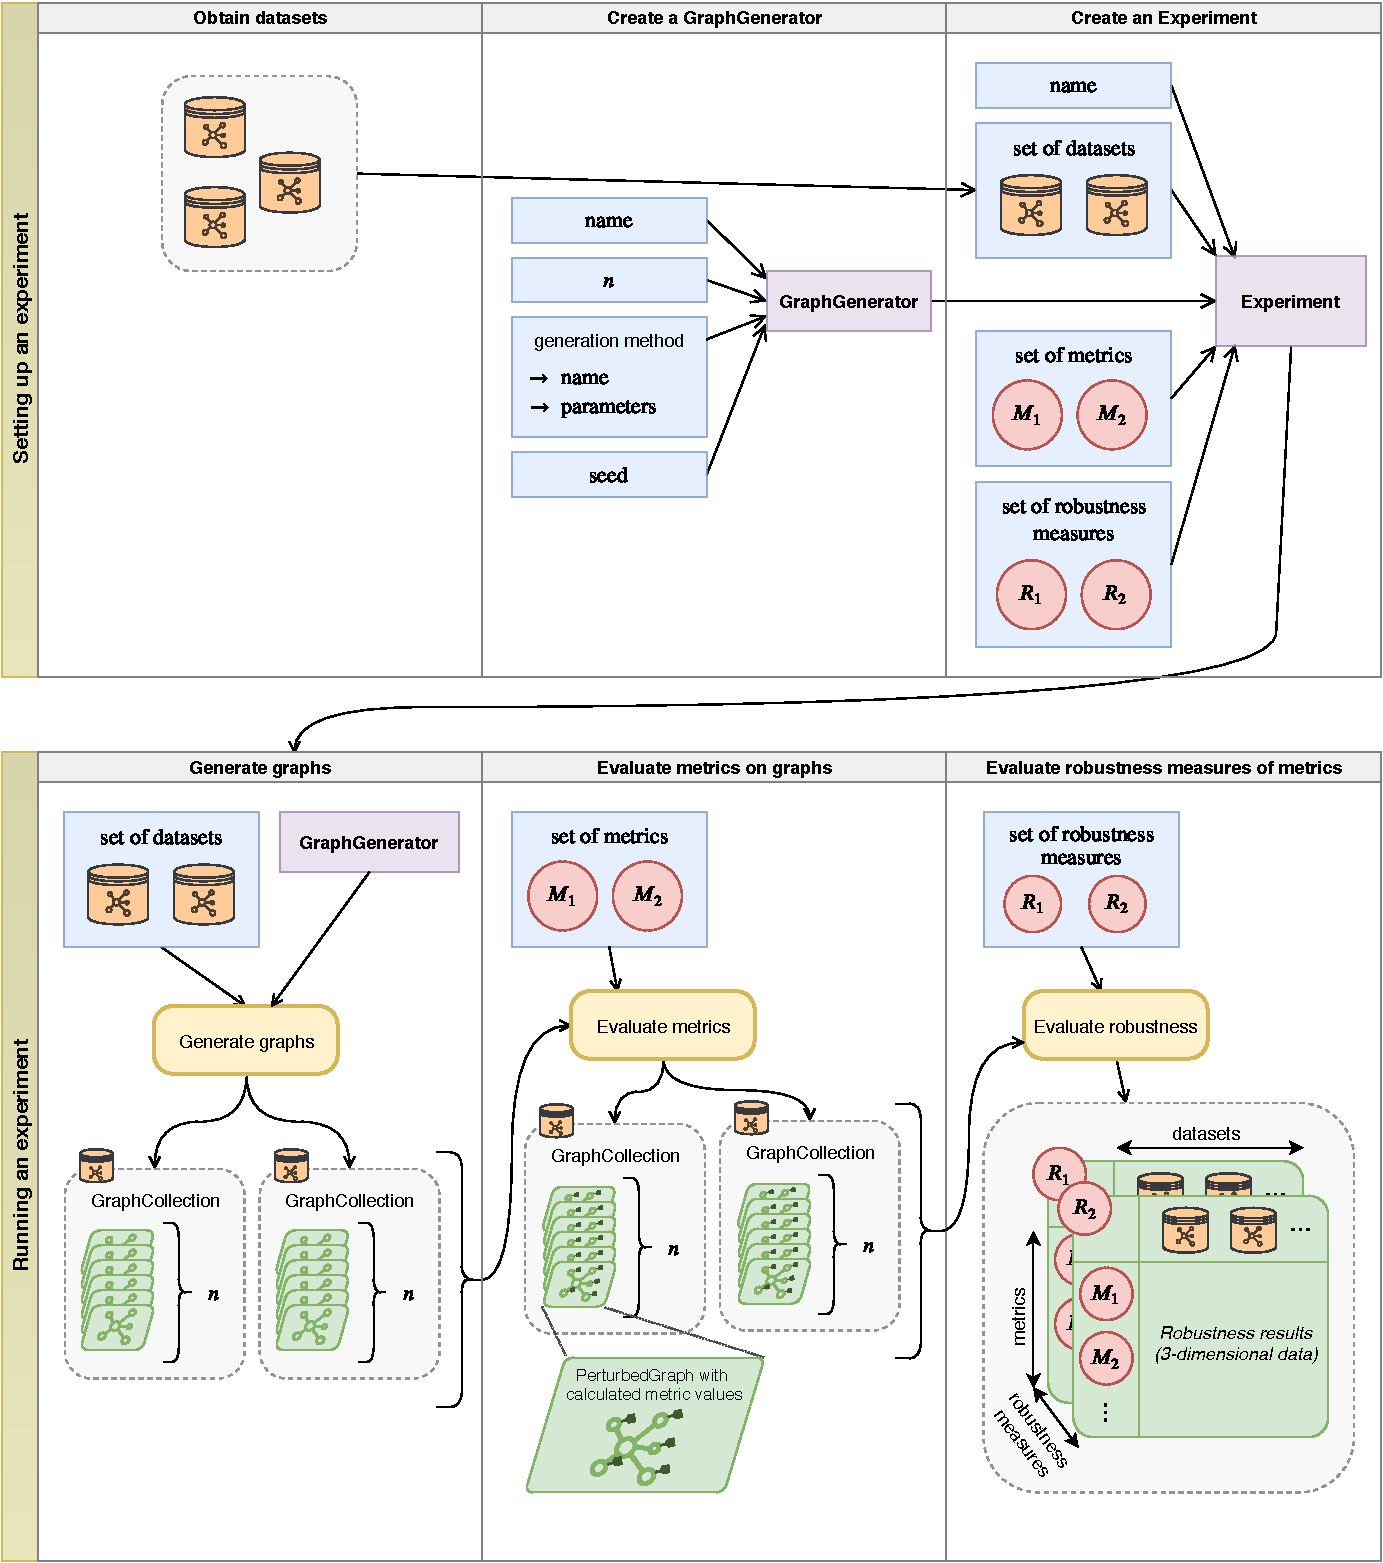
\includegraphics[width=\linewidth]{main_data_flow.pdf}
    \definecolor{diag-orange}{HTML}{D1A77D}
    \definecolor{diag-blue}{HTML}{6C8EBF}
    \definecolor{diag-violet}{HTML}{9673A6}
    \definecolor{diag-red}{HTML}{B85450}
    \definecolor{diag-yellow}{HTML}{D6B656}
    \definecolor{diag-green}{HTML}{82B366}
    \caption{Diagram showing the data flow of an experiment, in two phases: 1. setting up an experiment (the user collects/inputs data), 2. running an experiment (the program is running the computations as described in \autoref{sec:main_pipeline}). The result is a 3-dimensional data with a calculated robustness value for each from \textsl{datasets, metrics, robustness measures}.}\label{fig:main_data_flow}
    \footnotesize\justify\vspace{-0.4\baselineskip}
    Legend: \textcolor{diag-orange}{orange} -- datasets; \textcolor{diag-blue}{blue} -- user input; \textcolor{diag-violet}{violet} -- user-defined persisted entity; \textcolor{diag-red}{red} -- program-defined operations; \textcolor{diag-yellow}{yellow} -- processes; \textcolor{diag-green}{green} -- program-generated output; arrows $\rightarrow$ represent the flow of data.
\end{figure}


Running the experiment is a computationally intensive task, mainly due to metric evaluation (which certainly depends on the chosen metrics).
To mitigate this, I employed the following:
\begin{itemize}[topsep=5pt]
    \item Optimised the program for computation speed by applying performance engineering principles
    \item Allow parallel computation
    \item I ran extensive experiments on a high-performance computing facility (from \autoref{sec:computing_cluster})
\end{itemize}

\autoref{fig:main_data_flow} illustrates the flow of data across the above-mentioned steps.

\subsection{Loading datasets}

Datasets are located, and are expected to be located, in the `data' directory in the \graffs's working directory (i.e. where the program is run).
Each sub-directory represents a dataset identified by the sub-directory's name.
\graffs supports loading files of two different types of files:

\begin{description}[itemsep=\zerospace]
    \item \hyperref[sec:edge_files]{\textbf{Edge files}} -- text format with each line containing a pair of adjacent nodes
    \item \hyperref[sec:rdata_files]{\textbf{\texttt{RData} files}} -- binary files that store objects created in the R language~\cite{RCoreTeamLanguageEnvironmentStatistical2009}
\end{description}

\begin{figure}
\begin{tikzpicture}%
\draw[color=black!60!white]
\FTdir(\FTroot,i0,data){
\FTdir(i0,i1,citation){
\FTfile(i1,edges.txt)
\FTfile(i1,info.txt)
}
\FTdir(i0,i2,ecoli){
\FTfile(i2,info.txt)
\FTfile(i2,string\_ecoli\_data.RData)
}
\FTdir(i0,i3,facebook){
\FTfile(i3,edges.txt)
\FTfile(i3,info.txt)
}
\FTdir(i0,i4,pvivax){
\FTfile(i4,info.txt)
\FTfile(i4,string\_pvivax\_data.RData)
}
\FTdir(i0,i5,test){
\FTfile(i5,edges.txt)
}
\FTdir(i0,i6,yeast){
\FTfile(i6,info.txt)
\FTfile(i6,string\_yeast\_data.RData)
}
};
\end{tikzpicture}

\caption{An example structure of the \texttt{data} directory}
\label{fig:data_dir_structure}
\end{figure}


In each dataset's directory, the program looks for a file that ends with either \texttt{.RData} or \texttt{.txt}, in this order.
Datasets may additionally contain an \texttt{info.txt} file holding a human-readable description of the dataset (that is printed in the command-line interface when the dataset is loaded).
\autoref{fig:data_dir_structure} shows an example directory structure.

The \texttt{GraphLoader} abstract class (\autoref{lst:code_graphloader}) is to be implemented in both cases.
\lstinputlisting[label={lst:code_graphloader}, caption={The \texttt{GraphLoader} abstract class, providing a contract for implementations to load graphs}, float=ht, language=Kotlin, firstline=6]{GraphLoader.kt}

\subsubsection{Edge files}\label{sec:edge_files}

A common pure format of storing network structure (without any metadata) is to list the edges line by line, with each line containing unique identifiers of two nodes.
The set of nodes is then implicitly defined by the set of all distinct node identifiers present in the file.

However, different dataset sources (\autoref{sec:datasets}) provide \texttt{.txt} edge files with the content in different formats.
Some edge files contain a header, \texttt{\#comments}, or a third number in each line representing the edge's weight (for \hyperref[sec:scored_networks]{scored networks}).
\autoref{fig:edge_file_examples} shows a number of example edge files that should be accepted by \graffs.

%! Suppress = Ellipsis
% @formatter:off
\begin{savenotes}
\begin{figure}[!ht]
\caption{Three examples of dataset files containing one edge definition per line.}\label{fig:edge_file_examples}
\begin{minipage}[t]{.12\textwidth}
\raggedright\footnotesize \texttt{edges.txt}, a~sample graph file
\begin{lstlisting}
0 1
0 2
0 3
0 4
0 5
0 6
0 7
1 2
1 4
1 5
1 8
1 9
1 10¦\Suppresslinenumbers¦
...
\end{lstlisting}\Reactivatelinenumbers
\end{minipage}\hspace*{0.8cm}%
\begin{minipage}[t]{.36\textwidth}
\footnotesize \texttt{Cit-HepTh.txt} citation network from Stan\-ford Large Network Data\-set Col\-lec\-tion\footnote{URL: \url{https://snap.stanford.edu/data/cit-HepTh.html}}
\begin{lstlisting}
# Directed graph (each unordered pair of nodes is saved once): Cit-HepTh.txt
# Paper citation network of Arxiv High Energy Physics Theory category
# Nodes: 27770 Edges: 352807
# FromNodeId	ToNodeId
1001	9304045
1001	9308122
1001	9309097
1001	9311042
1001	9401139¦\Suppresslinenumbers¦
...
\end{lstlisting}\Reactivatelinenumbers
\end{minipage}\hspace*{0.8cm}%
\begin{minipage}[t]{0.41\textwidth}
\footnotesize \texttt{362663.protein.links.v11.0.txt} \\(Escherichia coli) from the STRING data\-base\footnote{URL: \url{https://string-db.org/cgi/download.pl?species_text=Escherichia+coli+536}}
\begin{lstlisting}
protein1 protein2 combined_score
362663.ECP_0001 362663.ECP_0006 518
362663.ECP_0001 362663.ECP_0003 606
362663.ECP_0001 362663.ECP_0002 606
362663.ECP_0001 362663.ECP_0005 518
362663.ECP_0001 362663.ECP_0004 606
362663.ECP_0002 362663.ECP_0798 158
362663.ECP_0002 362663.ECP_1284 175
362663.ECP_0002 362663.ECP_1357 170
362663.ECP_0002 362663.ECP_0918 621
362663.ECP_0002 362663.ECP_1773 175
362663.ECP_0002 362663.ECP_2824 342
362663.ECP_0002 362663.ECP_4415 320¦\Suppresslinenumbers¦
...
\end{lstlisting}\Reactivatelinenumbers
\end{minipage}%
\hspace*{-0.5cm}
\end{figure}
\end{savenotes}
% @formatter:on


One way would be to distinguish different formats by the file extension, or with additional meta information.
However, one of the goals for \graffs is to make it as versatile as possible, thus not requiring the user to manually specify a dataset's type or source is welcome.

Hence, I implemented \texttt{FileSourceEdgeOptionalWeight} parser, extending GraphStream's \texttt{FileSourceEdge} simple LR parser, to allow the following:
\begin{itemize}[topsep=5pt]
    \item Modify the grammar to correctly parse node IDs containing dots (\texttt{.}), such as \texttt{362663.ECP\_0001} (to allow datasets from the STRING database)
    \item Ignore comment lines starting with \texttt{\#} or \texttt{\%} characters
    \item Ignore headers starting with the string \texttt{protein1} (included in graph files downloaded from the STRING database)
    \item Recognise if a line has 3 tokens instead of 2, in which case parse and store it as the weight of the edge
\end{itemize}

\subsubsection{RData files}\label{sec:rdata_files}

The Paper~\cite{Bozhilova2019} provides the dataset files that were used in their research\footnote{Available at \url{http://opig.stats.ox.ac.uk/resources}}, in the \texttt{RData} format, a binary file capturing a session of the R language, storing objects from the \texttt{igraph} R package.

To load such files, an option is to convert them manually into another \graffs-readable format, or let \graffs call R to do this conversion under the hood.
To make \graffs as versatile as possible and not require the R software environment to be installed on the client's computer, I employed the Renjin library\footnote{Rejin official website: \url{https://www.renjin.org/}}, a \enquote{JVM-based interpreter for the R programming language}.
Renjin can execute R code (as well as load RData files) within Java, without the need to install any additional platform.

When an RData file is to be loaded in \graffs, a Renjin engine starts under the hood and loads desired file.
If an object whose name ends with \texttt{.df}\footnotemark{} is found, it is converted into a GraphStream's \texttt{Graph} object.
\footnotetext{This is to follow convention from \url{https://github.com/lbozhilova/measuring_rank_robustness/blob/c39bfed/data_prep.R}}

\subsection{Generating graphs}

First, there is the \texttt{GraphProducer} interface, which has a single method\footnotemark{}:\\ \texttt{fun produce(sourceGraph: Graph, n: Int): List<Deferred<PerturbedGraph>>}
\footnotetext{It returns a list of \texttt{Deferred} objects from the \texttt{kotlinx.coroutines} package, so that the generation can be parallelised at a higher level in the program using \textsl{Kotlin coroutines}, as described in \autoref{sec:kotlin_coroutines}.} \\
Each |GraphProducer| implementation provides a corresponding |GraphProducerFactory| object, defined as:
% @formatter:off
\begin{lstlisting}[language=Kotlin]
typealias GraphProducerFactory =
    (seed: Long, params: List<Number>, coroutineScope: CoroutineScope) -> GraphProducer
\end{lstlisting}
% @formatter:on

Further, \texttt{GraphGenerator}s (from \autoref{fig:data_model_classes_diagram}), which are stored in the database, have the \texttt{method} field referencing a \texttt{GraphProducer} to use.

Implementations of the methods for producing graphs as described in~\autoref{sec:perturbing_graphs} are straightforward.
Each generated graph is in some way a copy of the input graph, with some edges deleted.

\subsection{Evaluating metrics}

Metrics are classes (or rather, Kotlin |object|s) implementing the |Metric| interface, with a single method \texttt{fun evaluate(graph: Graph): MetricResult?}.

In the database, each |PerturbedGraph| entry stores a single serialised |Graph| object, whose nodes holds values for all metrics.
A metric's value at each node is stored in the node's attribute map.

An |Experiment| entry (those are created by the user) has a |Set<String>| field specifying which metrics to evaluate on each |PerturbedGraph|, and those metrics are again referenced by a |String| identifier.

\subsection{Metric robustness}

Similar to other concepts, robustness measure classes implement the |RobustnessMeasure| interface, with a single method |suspend fun evaluate(metric: MetricInfo, graphCollection: GraphCollection, metadata: GraphCollectionMetadata): Double|.

|MetricInfo| uniquely identifies the |Metric| whose robustness to calculate.
|GraphCollection| is an entity (from \autoref{fig:data_model_classes_diagram}) with a list of |PerturbedGraph|s of one dataset.
|GraphCollectionMetadata| provides cached\footnotemark{} access to intermediate results regarding the particular |GraphCollection| in the context of the current |Metric|, such as the \textsl{overall ranking} of the given metric over all the perturbed graphs (see \autoref{def:overall_ranking}).
\footnotetext{cached, as the overall ranking is calculated only once for each \texttt{GraphCollection} and each \texttt{Metric}, and used for more robustness measures}
Each |RobustnessMeasure| returns a single |Double| value, which is the numerical result, calculated as described in \autoref{sec:robustness_measures}.
The |evaluate| function has the |suspend| modifier so that it can suspend and finish asynchronously within the context of Kotlin coroutines (see \autoref{sec:kotlin_coroutines}).

\subsubsection*{Resolving ties}

An important detail when using ranking vectors (e.g. for the overall ranking) is specifying how ties are resolved.
According to the definition of ranking vector (\cref{def:ranking_vector}), if we have $v_1, v_2 \in V$ with $M(v_1) = M(v_2)$ for some metric $M$, then $\preceq$ is a valid ranking relation with either $v_1 \preceq v_2$ or $v_2 \preceq v_1$.
In The Paper, such ties were resolved \enquote{at random, independently across different metrics and different thresholds}.
This may, however, lead to inappropriately lower robustness of metrics due to random oscillations of ranks of nodes, as well as a high degree of variability between results (especially for graphs with small number of nodes).

In \graffs, I assured that ties are resolved arbitrarily but deterministically and constantly across all metrics and thresholds, and even constantly across multiple (perturbed) graphs with the same nodes (see \cref{sec:perturbing_graphs} on perturbing graphs).
This follows the~\nameref{sec:reproducibility} principle set in~\nameref{sec:design-goals}.

\subsection{Visualising graphs \& producing figures}

\todo{todo}


\section{Parallelism using Kotlin coroutines}
\label{sec:kotlin_coroutines}

Kotlin supports a concept of \textsl{suspending functions}, i.e. functions which can pause their execution (storing its \textsl{current continuation}) and return the control of the flow back to its caller, and later continue by resuming the continuation at the suspension point.
The context in which a suspending function suspends, is called coroutine.
Coroutines are a well-known control abstraction in programming languages~\cite{MouraRevisitingCoroutines2009} that can easily be implemented in higher-order languages using continuations\cite{HaynesContinuationsCoroutines1984}.

Asynchronous computations, delays, or IO operations can be programmed as suspending calls, i.e. functions that are allowed to \textsl{suspend} (or \textsl{pause}) coroutine voluntarily, and return the control back to the caller, then continue whenever their \textsl{continuation} is resumed (or invoked).

Coroutines can be used even within a single thread, and so allow a concurrent execution.
In the case of \graffs, however, we are interested in running computation in parallel, to utilise the power of multiple CPU cores.
A simple solution in Java would be to use |Thread|s, or a library working with threads directly.
This would work but it's heavyweight, not very expressive and not safe (e.g. a failure of an operation in one thread will not automatically cancel following or related tasks in other threads, unless this safety is implemented manually).
Another option is to use job queueing and an abstract multi-threaded executor, but then specifying inter-task execution order constraints would still be verbose, and running jobs would not be abstracted away from the code defining the jobs.

Kotlin coroutines are \textsl{lightweight threads} -- spawning coroutines is fast and cheap~\cite{AriasFunctionalKotlinExtend2018}.
They have a similar life cycle and are executed within regular threads, although they are not bound to them~\cite{TorresLearningConcurrencyKotlin2018}.
Coroutines allow executing suspending functions.

Suspending functions in Kotlin, when compiled to Java bytecode, are regular functions accepting |Continuation<Int>| as one of the arguments.
The |async| function (or its alternatives) takes a suspending function, creates an asynchronous coroutine executing the function and immediately returns its future result (as |Deferred<T>|).
Then the |await| suspending function called on a |Deferred| object waits for the resulting value without blocking, and resumes when the deferred computation is complete.

Kotlin also provides other means to synchronise coroutines, such as using mutual exclusion or actors, when needed in a parallel execution.
Mutexes are used to ensure synchronised access when persisting entities in the database.

\todo{diagram similar to \url{https://s3.amazonaws.com/kukuruku-co/uploads/images/00/17/75/2016/10/09/126426.png}}

The following parts of \graffs use parallel programming with coroutines:
\begin{itemize}[topsep=5pt]
    \item Generating graphs
    \item Evaluating metrics on graphs

    Each |Graph| is treated individually without the need to synchronise across them, however, evaluation of metrics within one |Graph| is sequential as the GraphStream library does not support parallel access.
    \item Evaluating robustness, including calculating overall ranks, which must be calculated for each |GraphCollection| before any robustness measure is evaluated on it
    \item Generating various figures, for which an intermediate
\end{itemize}


\section{Command line interface}\label{sec:cli}

The \graffs tool is built as a program with rich and intuitive command-line interface.
The program is pre-packaged in a \texttt{.jar} file, built for Java 8 or higher, so running it involves running the shell command:
% @formatter:off
\begin{lstlisting}[language=bash,style=light]
java -jar graffs.jar [ARGS]
\end{lstlisting}
% @formatter:on

Clikt is a \enquote{multiplatform command line interface parsing for Kotlin}\footnote{Available at \url{https://github.com/ajalt/clikt}} library that I used for defining commands, their behaviour, description, and hierarchy, in a structured way.
The library utilises a number of features of the Kotlin language, such as delegated properties, extension functions, and default arguments, resulting in a cleaner code that uses the library.

The \graffs tool provides many commands (loading datasets, creating and accessing graph generators, creating and running experiments, and so on).
Commands are grouped based on their context and the objects that they operate on, and can further have sub-commands.
Those are together structured in a tree-like hierarchy.
The hierarchy is shown in \autoref{fig:cli_commands_hierarchy}.

\begin{figure}
\caption{Hierarchy of supported command-line interface commands, and their brief description}
\label{fig:cli_commands_hierarchy}
\begin{flushleft}
\setlength{\DTbaselineskip}{11pt}
\small
\dirtree{%
.1 graffs \scriptsize \dotfill\ \begin{minipage}[t]{10.6cm}Tool for evaluating Graph Metric Robustness\end{minipage}.
.2 dataset \scriptsize \dotfill\ \begin{minipage}[t]{10.6cm}Access available datasets\end{minipage}.
.3 list \scriptsize \dotfill\ \begin{minipage}[t]{10.6cm}List all datasets available in the `data` directory\end{minipage}.
.3 load \scriptsize \dotfill\ \begin{minipage}[t]{10.6cm}Check if datasets can be loaded from the `data` directory\end{minipage}.
.3 download-demos \scriptsize \dotfill\ \begin{minipage}[t]{10.6cm}Download datasets for demonstration\end{minipage}.
.3 viz \scriptsize \dotfill\ \begin{minipage}[t]{10.6cm}Visualise graph\end{minipage}.
.2 metric \scriptsize \dotfill\ \begin{minipage}[t]{10.6cm}Access available metrics\end{minipage}.
.3 list \scriptsize \dotfill\ \begin{minipage}[t]{10.6cm}List available graph metrics\end{minipage}.
.2 generator \scriptsize \dotfill\ \begin{minipage}[t]{10.6cm}Create or list graph generators\end{minipage}.
.3 list \scriptsize \dotfill\ \begin{minipage}[t]{10.6cm}List available graph generators\end{minipage}.
.3 create \scriptsize \dotfill\ \begin{minipage}[t]{10.6cm}Create a new graph generator description\end{minipage}.
.3 remove \scriptsize \dotfill\ \begin{minipage}[t]{10.6cm}Remove a graph generator\end{minipage}.
.2 experiment \scriptsize \dotfill\ \begin{minipage}[t]{10.6cm}Manage experiments (evaluating metrics on generated graphs)\end{minipage}.
.3 list \scriptsize \dotfill\ \begin{minipage}[t]{10.6cm}List created experiments and their properties\end{minipage}.
.3 create \scriptsize \dotfill\ \begin{minipage}[t]{10.6cm}Create an experiment\end{minipage}.
.3 change \scriptsize \dotfill\ \begin{minipage}[t]{10.6cm}Change an existing experiment\end{minipage}.
.3 clone \scriptsize \dotfill\ \begin{minipage}[t]{10.6cm}Create a new experiment using parameters of existing experiment\end{minipage}.
.3 remove \scriptsize \dotfill\ \begin{minipage}[t]{10.6cm}Remove an experiment, all its generated graph and any computed results\end{minipage}.
.3 run \scriptsize \dotfill\ \begin{minipage}[t]{10.6cm}Run an experiment\end{minipage}.
.3 prune \scriptsize \dotfill\ \begin{minipage}[t]{10.6cm}Remove generated graphs and calculated robustness values of an experiment\end{minipage}.
.2 plot \scriptsize \dotfill\ \begin{minipage}[t]{10.6cm}Plot results\end{minipage}.
.3 rank-similarity.
.2 db \scriptsize \dotfill\ \begin{minipage}[t]{10.6cm}Manage the underlying database\end{minipage}.
.3 test \scriptsize \dotfill\ \begin{minipage}[t]{10.6cm}Test the database connection\end{minipage}.
.3 drop \scriptsize \dotfill\ \begin{minipage}[t]{10.6cm}Reset the database schema and contents\end{minipage}.
}
\end{flushleft}
\end{figure}


Further, \autoref{lst:graffs_cli_examples} shows an example output of some of the commands.

\lstinputlisting[label={lst:graffs_cli_examples}, caption={A demonstration of the help text printed by the command-line tool}, float, basicstyle=\ttfamily\color{black}\fontsize{8pt}{8pt}\selectfont,]{graffs-help.txt}

\todo{Describe Clikt features such as command completion}




    \chapter{Evaluation}\label{ch:evaluation}
    \section{Reliability of \graffs}

- why is~\nameref{sec:randomly_removing_edges} as good as thresholding?
maybe apply Randomly removing edges to scored networks and see the difference of robustness


\section{Reproducing results}


\section{Extending to further datasets}


\section{(Predicting metric stability)}


\section{Releasing \graffs}
\subsection{Licensing}



    \chapter{Conclusion}\label{ch:conclusion}
    %

    %TC:ignore

%    \chapter{(Scratch)}

\section{Libraries / frameworks}
I used a number of libraries to help with concepts as described in the subsections below.

\subsection{Graph representation and algorithms}

I reviewed the most developed and maintained libraries that allow representing graphs.

\begin{itemize}
    \item \textbf{JGraphT} (\url{https://jgrapht.org})

    \enquote{a Java library of graph theory data structures and algorithms}

    Probably the most popular Java library for working with graphs.
    It is algorithm-focused, however, the algorithms relate mostly to walking on graph nodes and are not for evaluating graph metrics.
    JGraphT also does doesn't come with visualisations.

    \item \textbf{GraphStream} (\url{http://graphstream-project.org/})



    \item \textbf{Graphviz} (\url{https://www.graphviz.org/})

    \enquote{open source graph visualization software}

    Graphviz is specifically made for creating visual graphs, diagrams and abstract networks, for visual interfaces.
    Not suitable for this project.
\end{itemize}

Taking pros and cons of the above-mentioned graph libraries into account, I chose to use \textbf{GraphStream}.

GraphStream consists of 3 modules:

\begin{enumerate}
    \item \texttt{gs-core} Core implementation of the graph library
    \item \texttt{gs-algo} Various algorithms from graph theory
    \item \texttt{gs-ui} Components for visualising graphs
\end{enumerate}

\subsection{Batch Job processing framework}

As evaluation of metrics on a huge number of generated graphs takes a lot of computational resources, \texttt{graffs} runs on a framework that supports distributed computations.

\begin{itemize}
    \item Apache Flink (\url{https://flink.apache.org})

    \enquote{Stateful Computations over Data Streams}

    Slightly less popular framework for distributed streaming and data processing.
    \item Apache Samza (\url{http://samza.apache.org/})

    \enquote{open-source near-realtime, asynchronous computational framework for stream processing}

    The usage seems to be relatively heavyweight and relies on Apache Kafka and Zookeeper.
    \item Apache Storm (\url{https://storm.apache.org/}) *

    \enquote{open source distributed realtime computation system}

    (a good possible alternative.
    See \url{https://storm.apache.org/releases/2.1.0/Tutorial.html})
    \item Apache Akka (\url{https://akka.io/})

    \enquote{toolkit and runtime simplifying the construction of concurrent and distributed applications on the JVM}
    \item Apache Hadoop (\url{https://hadoop.apache.org/})

    \enquote{framework that allows for the distributed processing of large data sets across clusters}
    \item Apache Heron (\url{https://apache.github.io/incubator-heron/})

    \enquote{realtime, distributed, fault-tolerant stream processing engine from Twitter}
    \item Apache Beam (\url{https://beam.apache.org/})

    \enquote{open source unified programming model to define and execute data processing pipelines}
    \item Apache NiFi (\url{https://nifi.apache.org/})

    \enquote{supports powerful and scalable directed graphs of data routing, transformation, and system mediation logic}
    \item Spring Boot (\url{https://spring.io/projects/spring-boot})

    \enquote{makes it easy to create stand-alone, production-grade Spring based Applications}
    \item Apache Apex (\url{https://apex.apache.org/})

    \enquote{Enterprise-grade unified stream and batch processing engine} (now a retired project)
    \item Apache Spark™

    \enquote{unified analytics engine for large-scale data processing}

    Spark is one of the most maintained framework for computation-heavy tasks
\end{itemize}

\subsection{Database}

\subsubsection{Database backend}

For simplicity, the H2 database system will be used, which can store a database in a single file.
A good alternative would be a MySQL installation.

\subsubsection{Object-relational mapping (ORM) library}

For robustness and simplicity of usage, \texttt{graffs} uses Java Persistence API (JPA) to help persist Java objects in the database as well as query them.
The API is Java classes and methods, so it abstracts away any queries in the native language of the database (such as SQL).

The \texttt{Hibernate} library (\url{http://hibernate.org/}) is an implementation of JPA that I used for the project.
It hides the underlying data storage system, as well as creating schema for the underlying database.
Schema is derived from Java classes (entities) defined in the source code.

Hibernate can also seamlessly connect to the H2 backend.

\subsection{CLI processing}

The \texttt{Clikt} library helps write the command line interface classes in a structured way.
Clikt is written in Kotlin and works especially well with Kotlin code as it leverages many of its features.
Further details of how I developed the command-line interface is in the~\nameref{ch:implementation} chapter.

\subsection{Apache Libraries}

\begin{itemize}
    \item Apache Commons Configuration:

    \url{https://commons.apache.org/proper/commons-configuration/}
    \item Apache Commons Compress:

    \url{https://commons.apache.org/proper/commons-compress/}
    \item Apache Commons CSV: \url{https://commons.apache.org/proper/commons-csv/}
    \item Apache Commons Logging:

    \url{https://commons.apache.org/proper/commons-logging/}
    \item Apache Commons Math: \url{https://commons.apache.org/proper/commons-math/}
    \item Apache Commons Pool: \url{https://commons.apache.org/proper/commons-pool/}
    \item Apache Commons Statistics:

    \url{https://commons.apache.org/proper/commons-statistics/}
\end{itemize}


\section{Terms and definitions}

I will loosely clarify, concretise or define the following terms:

\begin{description}
    \item[Graph]
    By graph, I mean a mathematical model of nodes connected by edges, from graph theory.
    Graphs is this work are implicitly \textbf{undirected}, if not stated otherwise.
    Nodes and edges may have values.

    \item[Metric of a graph]
    or graph metric, or just metric (in some contexts: measure), is a function of graphs.
    A metric may return a single value, or multiple values, such as for each node or each edge.
    Values are not necessarily numerical.

    \item [Dataset]
    In the context of this work, a dataset is a graph (alternatively a collection of graphs) that has a semantic meaning.
    For example, it may be known what source the graph came from, such as a social network.

    \item[Perturbation of a graph]
    Any change to the input graph resulting in a new graph (such as deleting a small percentage of edges), along with a mapping between nodes and edges of the original graph that have been preserved in the produced graph.

    \item[Generated graph]
    A graph that was produced by perturbing a dataset

    \item[Robustness of graph metric]
    A property of a graph metric, determining how sensitive to some perturbations in the input graph the metric is, i.e. how much the metric value(s) will change with small changes in the input graph.
    Robustness of a metric may depend on the kind of graph it is used on.
\end{description}

The~\nameref{ch:implementation} chapter further explain in detail terms \textbf{graph perturbations}, \textbf{metric value change} as well as \textbf{robustness}.


\section{Tools used}

% IntelliJ - Kotlin, JPA, Gradle, LaTex, figures
% Zotero
% MiKTeX (XeLaTeX), BibTex
% word count script
% SumatraPDF
% draw.io
% Inkscape
% H2
% JPA / Java EE plugin
% Hibernate framework
% Git, GitHub
% Draw.io
% Envato elements / graphics / icons



    %%%%%%%%%%%%%%%%%%%%%%%%%%%%%%%%%%%%%%%%%%%%%%%%%%%%%%%%%%%%%%%%%%%%%
    % the bibliography
    %\addcontentsline{toc}{chapter}{Bibliography}
    %\bibliographystyle{ieeetr}
    %\bibliography{refs}
    \printbibliography[heading=bibintoc]

    %%%%%%%%%%%%%%%%%%%%%%%%%%%%%%%%%%%%%%%%%%%%%%%%%%%%%%%%%%%%%%%%%%%%%
    % the appendices
    \appendix

    \chapter{Mathematical definitions}\label{ch:math_definitions}

\section{Graph theory}

Standard definitions of relevant concepts from graph theory, based mostly on \textsl{A first course in network theory}~\cite{Estrada2017}.

\begin{definition}[Graph]
    Let $V$ be a finite set of $n$ nodes (or vertices), and let $E \subseteq V \times V$ be a set of edges.\\
    A \textbf{graph} $G$ is a pair $(V, E)$.\\
    $V$ is the \textbf{node set} of $G$, and $E$ is the \textbf{edge set} of $G$.
\end{definition}

\begin{definition}[Graph properties]
    \begin{itemize}[leftmargin=*]
        \item $G$ is \textbf{reflexive} iff $\forall v \in V.\ (v, v) \in E$
        \item $G$ is \textbf{anti-reflexive} iff $\forall v \in V.\ (v, v) \notin E$
        \item $G$ is \textbf{undirected} (or equally \textbf{symmetric}) iff $\forall v_1, v_2 \in V.\ (v_1, v_2) \in E \Rightarrow (v_2, v_1) \in E$
        \item $G$ is \textbf{directed} iff it is not undirected
        \item $G$ is a \textbf{simple graph} iff it is undirected and anti-reflexive
    \end{itemize}
\end{definition}

\begin{definition}[Relations on graphs]
    \begin{itemize}[leftmargin=*]
        \item $G' = (V', E')$ is a \textbf{subgraph} of $G = (V, E)$ iff $V' \subseteq V$ and $E' \subseteq E$
        \item Let $G_1 = (V_1, E_1)$ and $G_2 = (v_2, E_2)$, then $G_1 \cup G_2 = (V_1 \cup V_2, E_1 \cup E_2)$ is the \textbf{union} of the two graphs, and $G_1 \cap G_2 = (V_1 {\cap} V_2, E_1 {\cap} E_2)$ is the \textbf{intersection} of the two graphs.
    \end{itemize}
\end{definition}

\begin{definition_with_break}[Node adjacency]
    \begin{itemize}[leftmargin=*]
        \item In an undirected graph, $v_1$ is \textbf{adjacent} to $v_2$ iff $(v_1, v_2) \in E$
        \item A \textbf{loop} is an edge of the form $(v, v)$.
        Note that simple graphs have no loops.
        \item Define $\deg^-(v) = \left\lvert \Set{v' \in V}{(v', v) \in E} \right\rvert$ to be the \textbf{indegree} of $v$, and $\deg^+(v) = \left\lvert \Set{v' \in V}{(v, v') \in E} \right\rvert$ to be the \textbf{outdegree} of $v$, in other words, the number of incoming and outcoming edges, respectively.
        If the graph is undirected, then $\deg^-(v) = \deg^+(v) = \deg(v)$ is called \textbf{degree}.
        \item For $G = (V, E)$ with $V = \integersto{n}$, define $A = (a_{ij})$ to be the \textbf{adjacency matrix} of $G$ where
        \[ a_{ij} = \begin{cases}
                        1, & \textnormal{if}\ (i, j) \in E \\
                        0, & \textnormal{if}\ (i, j) \notin E
        \end{cases} \]
        for $1 \leq i, j \leq n$.

        Note that adjacency matrix of undirected graph is symmetric.
    \end{itemize}
\end{definition_with_break}

\begin{definition}[Connectedness]
    \begin{itemize}[leftmargin=*]
        \item $u, v$ are \textbf{connected nodes} is there exists a path between $u, v$ in $G$, i.e. if $(A^k)_{uv} = 1$ for some $k\in \mathbb{N}$.
        \item $G = (V, E)$ is \textbf{connected graph} if $\forall v_1, v_2 \in V. v_1, v_2$ are connected nodes.
        \item A subgraph $G' \subseteq G$ is a \textbf{(connected) component} iff $G'$ is a maximal connected subgraph of $G$.

        Note that all components of a graph are disjoint, therefore each node belongs to exactly one component.
    \end{itemize}

    \item A \textbf{giant component} of a graph is a single component that has more nodes than any other component of the graph.

    Note that a giant component may not exist if more components have the maximum number of nodes.
\end{definition}


\section{Ranking}

These definitions precede those in \cref{sec:ranking}.

\begin{definition}[Partial order]
    A binary relation $\sqsubseteq$ on some set $P$ is a \textbf{partial order} iff it is antisymmetric preorder, i.e.:
    \begin{itemize}
        \item $\forall a, b \in P.\ a \sqsubseteq a$ \tabto{7.3cm}(reflexivity)
        \item $\forall a, b, c \in P.\ (a \sqsubseteq b \wedge b \sqsubseteq c) \implies a \sqsubseteq c$ \tabto{7.3cm}(transitivity)
        \item $\forall a, b \in P.\ (a \sqsubseteq b \wedge b \sqsubseteq a) \implies a = b$ \tabto{7.3cm}(antisymmetry)
    \end{itemize}
\end{definition}

\begin{definition}[Total order]
    A binary relation $\sqsubseteq$ on some set $P$ is a \textbf{total order} iff it is a partial order and a connex relation, i.e.:
    \begin{itemize}
        \item $\forall a, b, c \in P.\ (a \sqsubseteq b \wedge b \sqsubseteq c) \implies a \sqsubseteq c$ \tabto{7.3cm}(transitivity)
        \item $\forall a, b \in P.\ (a \sqsubseteq b \wedge b \sqsubseteq a) \implies a = b$ \tabto{7.3cm}(antisymmetry)
        \item $\forall a, b \in P.\ a \sqsubseteq b \vee b \sqsubseteq a$ \tabto{7.3cm}(connexity, implies reflexivity)
    \end{itemize}
\end{definition}



\chapter{Kotlin figures}\label{ch:appendix_kotlin_figures}
% Kotlin architecture
% Program figures
% Project figures

\begin{figure}
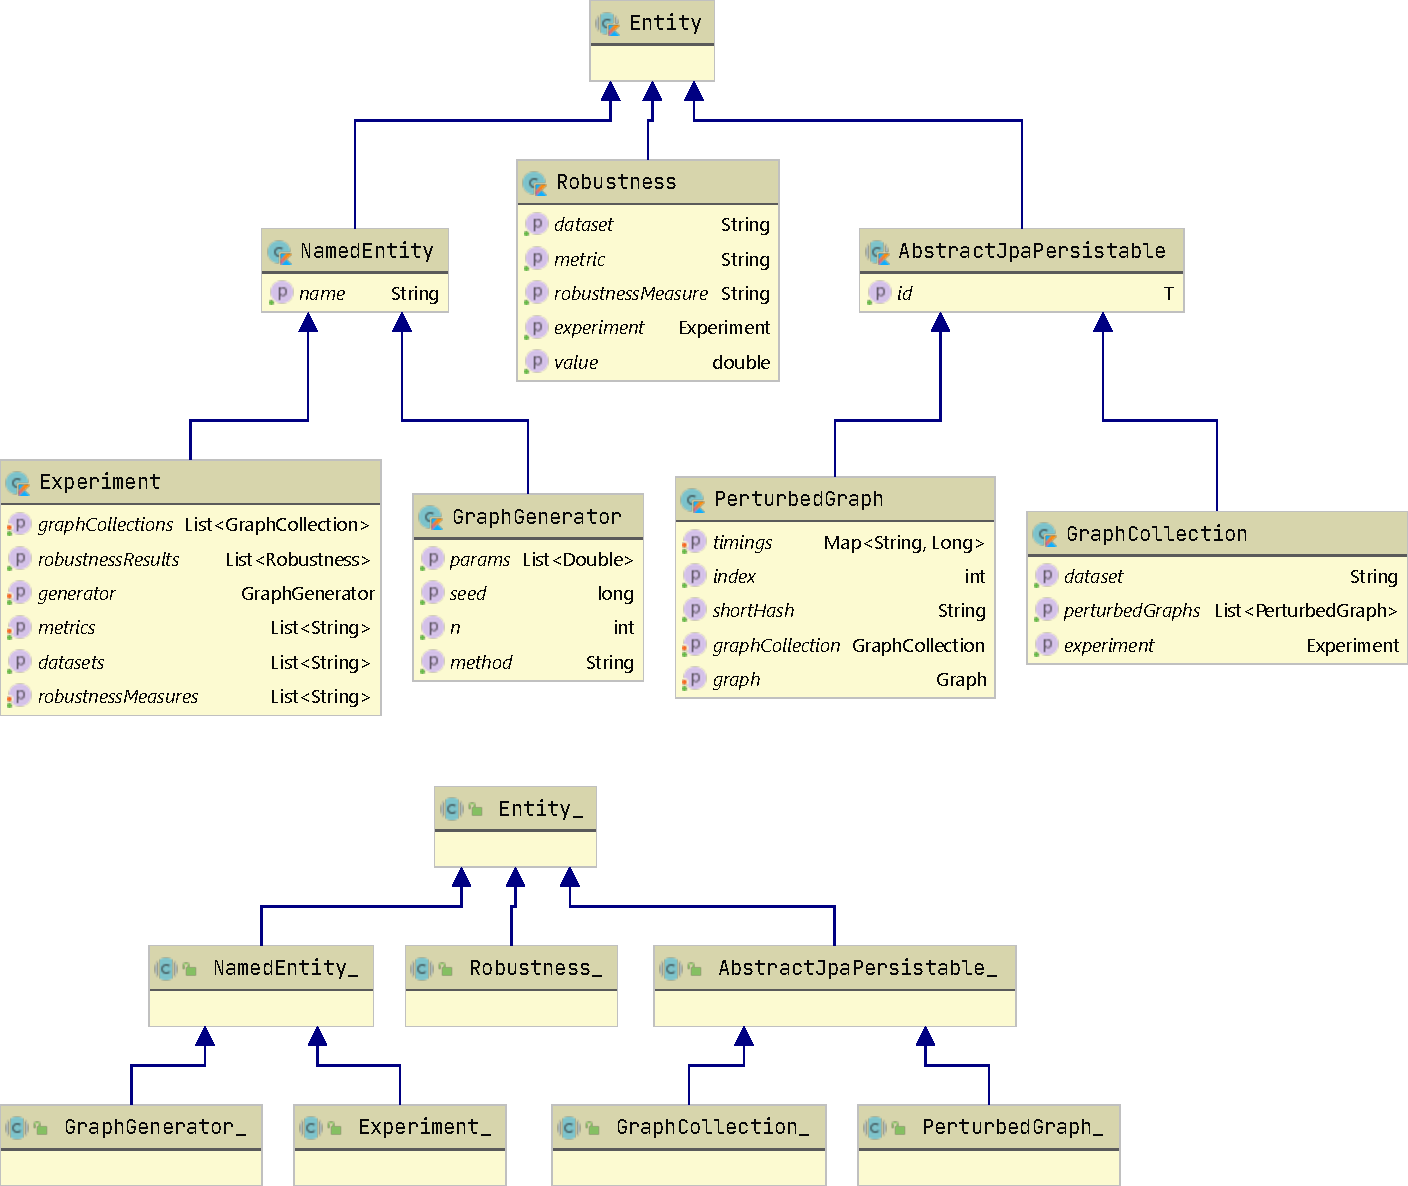
\includegraphics[width=\linewidth]{data_model_classes_diagram.pdf}
\caption{Inheritance hierarchy of the (Kotlin) classes underlying the persistence model presented in \autoref{fig:data_model_diagram}.
The arrows indicate \textsl{inheritance} (``is a'') relationships between classes.}
\label{fig:data_model_classes_diagram}
\end{figure}


\begin{figure}
    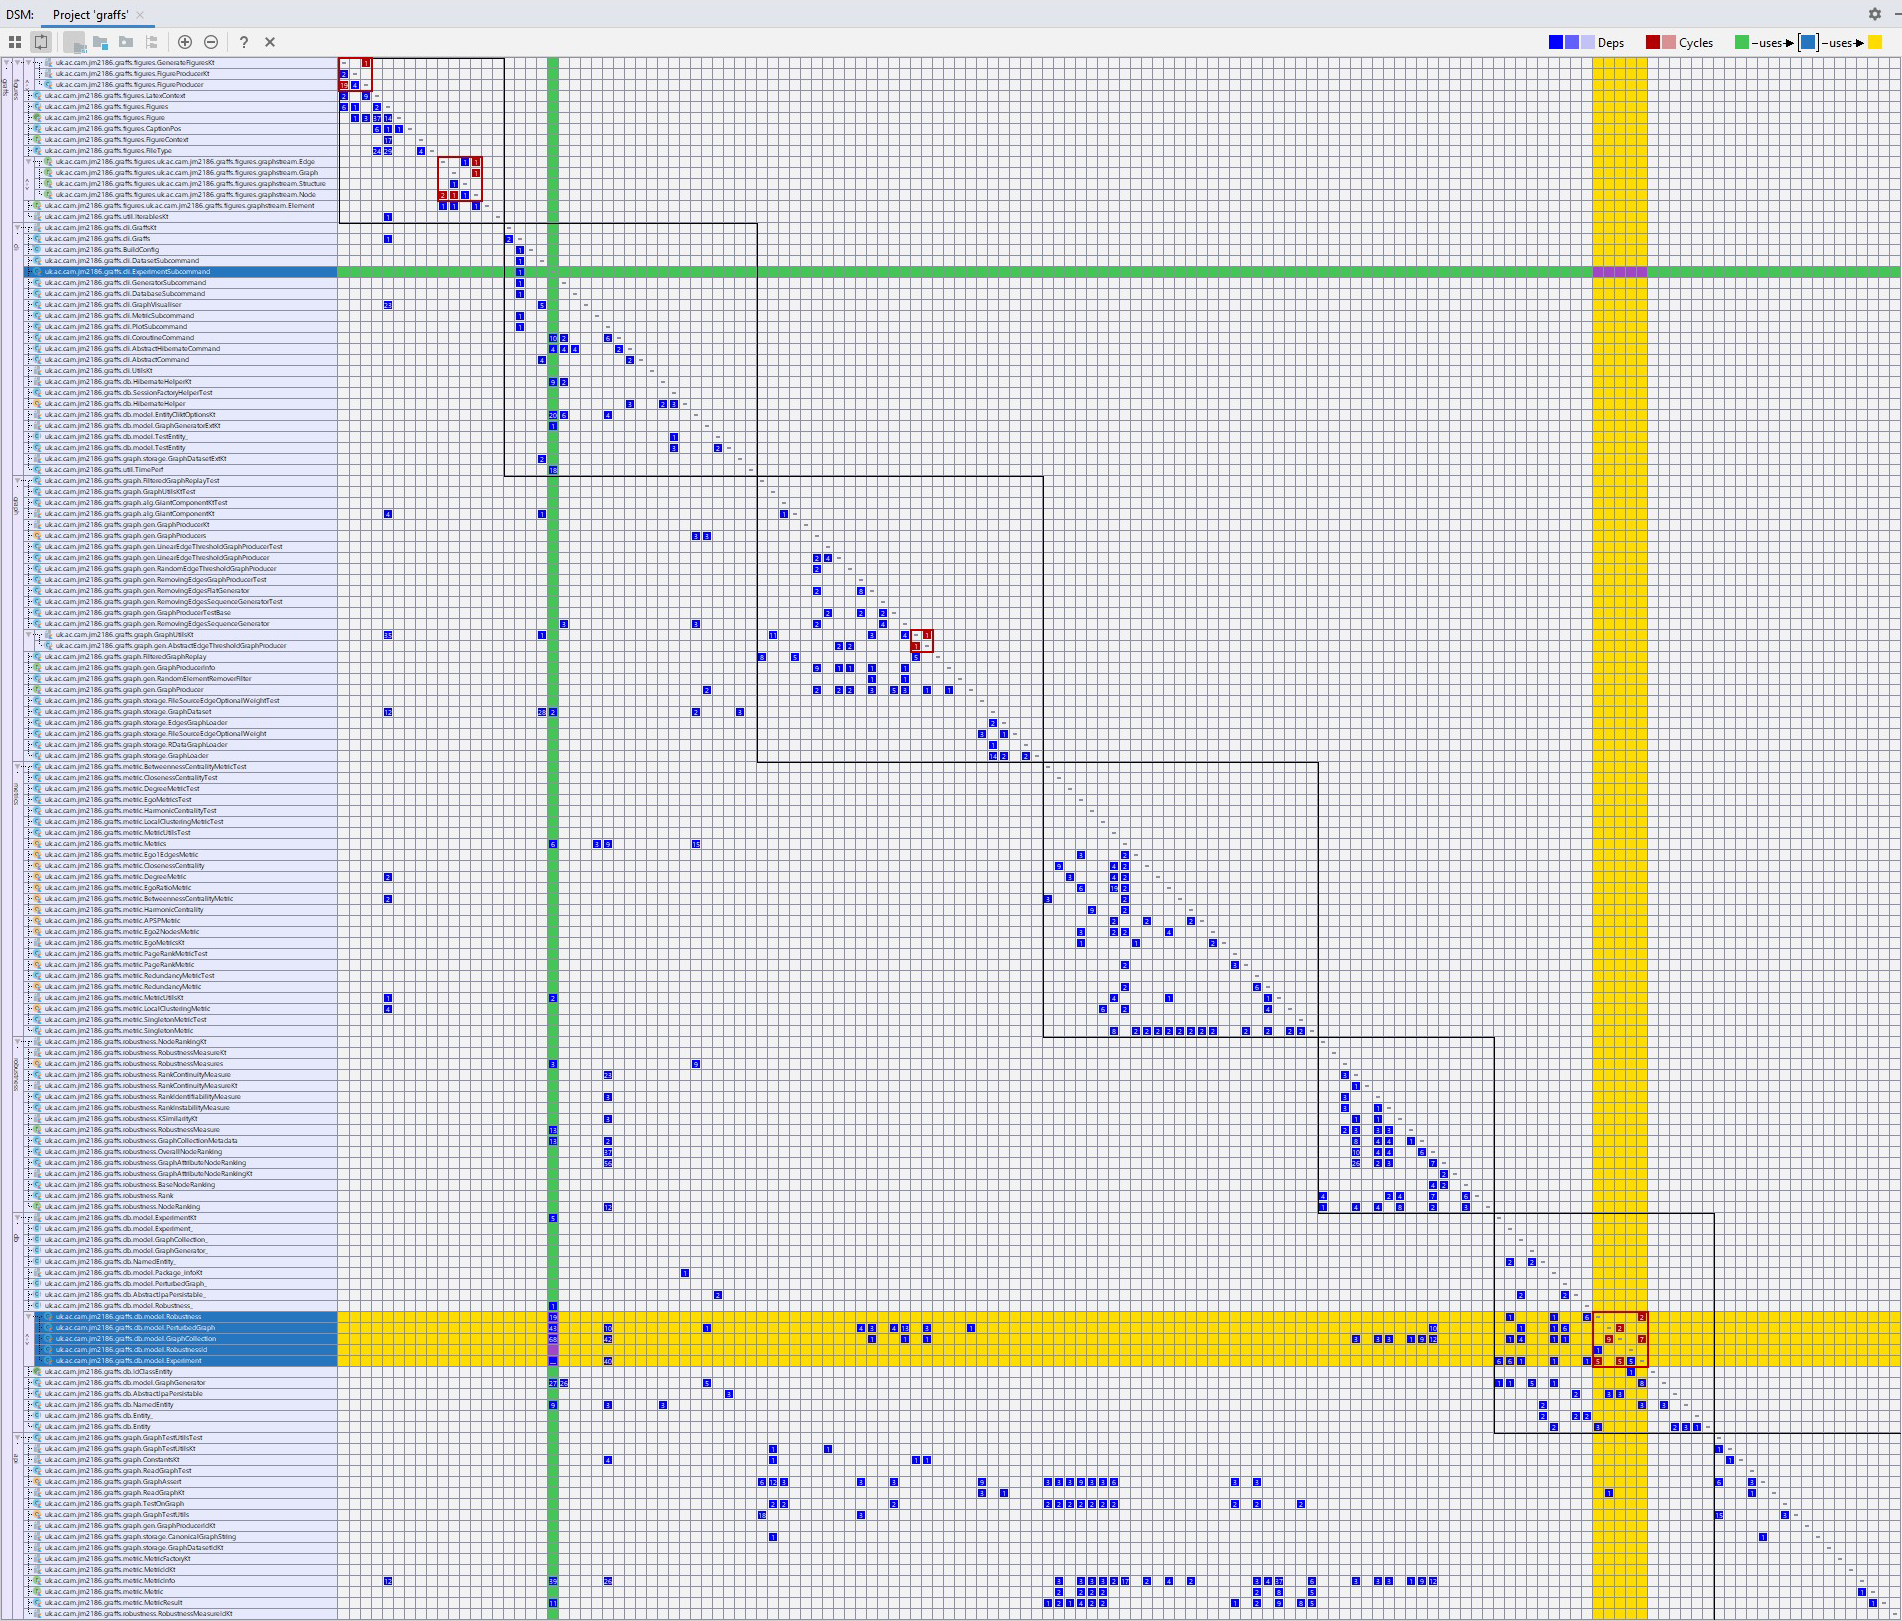
\includegraphics[width=\linewidth]{classes_dependency_matric.png}
    \caption{Dependency matrix between Kotlin files of \graffs (excluding tests), visualised by the IntelliJ IDEA editor.
    Each of the 7 groups corresponds to a module, namely: \texttt{figures}, \texttt{cli}, \texttt{graph}, \texttt{metric}, \texttt{robustness}, \texttt{db}, \texttt{api}.
    Cell in $i$-th row from the top and $j$-th column from the left corresponds to the dependency of $j$-th file on $i$-th file.
    Modules and files are ordered from more dependent (top) to less dependent (bottom).}
    \label{fig:classes_dependency_matrix}
    \footnotesize\justify\vspace{-0.4\baselineskip}
    The highlighted rows and columns show the directed dependency of the \texttt{ExperimentSubcommand} class (green), which provides the \texttt{graffs experiment} command-line subcommands, on the 5 JPA entity classes from \cref{fig:data_model_classes_diagram} (yellow).
\end{figure}


\clearpage

\lstinputlisting[label={lst:jpa_typed_query}, linerange=jpa_typed_query0-jpa_typed_query1, caption={A toy example of using typed Java Persistence API queries. Note the \texttt{Experiment\_} metamodel class generated from the \texttt{Experiment} entity by Hibernate, with (meta)fields corresponding to entities' fields.}, float, language=Kotlin]{listings.kts}

\lstinputlisting[label={lst:hibernate_load_entity}, linerange=hibernate_load_entity0-hibernate_load_entity1, caption={A toy example of Hibernate loading and persisting an \texttt{Experiment} object.}, float, language=Kotlin]{listings.kts}

\lstinputlisting[label={lst:graffs_cli_examples}, caption={A demonstration of the command-line help text of some subcommands, printed by \graffs}, float, basicstyle=\ttfamily\color{black}\fontsize{8pt}{8pt}\selectfont,]{graffs-help.txt}


\chapter{Robustness results}\label{ch:appendix_results}

\begin{table}[H]
\setlength{\tabcolsep}{5pt}\renewcommand{\arraystretch}{1}
\caption{RankContinuity of 7 metrics on 8 datasets (experiments \texttt{random-edges} and \texttt{unscored})}
\label{tab:robustness-continuity}
\scalebox{1}{
\begin{tabular}{|p{40mm}|ccc|ccccc|}
\toprule
{\small \textbf{RankContinuity}} & {\footnotesize \texttt{pvivax}} & {\footnotesize \texttt{ecoli}} & {\footnotesize \texttt{yeast}} & {\footnotesize \texttt{airports}} & {\footnotesize \texttt{collab}} & {\footnotesize \texttt{citation}} & {\footnotesize \texttt{facebook}} & {\footnotesize \texttt{internet}} \\
\midrule
                     Betweenness &                   {\small 1.00} &                  {\small 1.00} &                  {\small 1.00} &                     {\small 1.00} &                   {\small 0.70} &                     {\small 1.00} &                     {\small 0.83} &                     {\small 1.00} \\
                          Degree &                   {\small 1.00} &                  {\small 1.00} &                  {\small 1.00} &                     {\small 1.00} &                   {\small 1.00} &                     {\small 1.00} &                     {\small 1.00} &                     {\small 1.00} \\
                       Ego1Edges &                   {\small 1.00} &                  {\small 1.00} &                  {\small 1.00} &                     {\small 1.00} &                   {\small 1.00} &                     {\small 1.00} &                     {\small 1.00} &                     {\small 1.00} \\
                       Ego2Nodes &                   {\small 1.00} &                  {\small 1.00} &                  {\small 1.00} &                     {\small 1.00} &                   {\small 1.00} &                     {\small 1.00} &                     {\small 0.97} &                     {\small 1.00} \\
                 LocalClustering &                   {\small 0.23} &                  {\small 0.10} &                  {\small 0.07} &                     {\small 0.60} &                   {\small 0.33} &                     {\small 0.00} &                     {\small 0.07} &                     {\small 1.00} \\
                        PageRank &                   {\small 1.00} &                  {\small 1.00} &                  {\small 1.00} &                     {\small 1.00} &                   {\small 1.00} &                     {\small 1.00} &                     {\small 1.00} &                     {\small 1.00} \\
                      Redundancy &                   {\small 0.87} &                  {\small 1.00} &                  {\small 1.00} &                     {\small 1.00} &                   {\small 1.00} &                     {\small 0.73} &                     {\small 1.00} &                     {\small 1.00} \\
\bottomrule
\end{tabular}
}
\vspace*{2mm}
\caption{RankIdentifiability of 7 metrics on 8 datasets (experiments \texttt{random-edges} and \texttt{unscored})}
\label{tab:robustness-identifiability}
\scalebox{1}{
\begin{tabular}{|p{40mm}|ccc|ccccc|}
\toprule
{\small \textbf{RankIdentifiability}} & {\footnotesize \texttt{pvivax}} & {\footnotesize \texttt{ecoli}} & {\footnotesize \texttt{yeast}} & {\footnotesize \texttt{airports}} & {\footnotesize \texttt{collab}} & {\footnotesize \texttt{citation}} & {\footnotesize \texttt{facebook}} & {\footnotesize \texttt{internet}} \\
\midrule
                          Betweenness &                   {\small 0.93} &                  {\small 0.94} &                  {\small 0.94} &                     {\small 0.97} &                   {\small 0.81} &                     {\small 0.91} &                     {\small 0.83} &                     {\small 1.00} \\
                               Degree &                   {\small 0.99} &                  {\small 1.00} &                  {\small 0.99} &                     {\small 1.00} &                   {\small 0.97} &                     {\small 1.00} &                     {\small 0.98} &                     {\small 1.00} \\
                            Ego1Edges &                   {\small 0.94} &                  {\small 1.00} &                  {\small 0.95} &                     {\small 1.00} &                   {\small 0.98} &                     {\small 0.97} &                     {\small 0.98} &                     {\small 1.00} \\
                            Ego2Nodes &                   {\small 0.94} &                  {\small 0.97} &                  {\small 0.74} &                     {\small 0.92} &                   {\small 0.82} &                     {\small 0.86} &                     {\small 0.35} &                     {\small 1.00} \\
                      LocalClustering &                   {\small 0.09} &                  {\small 0.13} &                  {\small 0.34} &                     {\small 0.14} &                   {\small 0.29} &                     {\small 0.13} &                     {\small 0.07} &                     {\small 1.00} \\
                             PageRank &                   {\small 0.99} &                  {\small 0.97} &                  {\small 0.96} &                     {\small 1.00} &                   {\small 0.89} &                     {\small 0.99} &                     {\small 0.94} &                     {\small 1.00} \\
                           Redundancy &                   {\small 0.85} &                  {\small 0.98} &                  {\small 0.98} &                     {\small 0.92} &                   {\small 0.97} &                     {\small 0.80} &                     {\small 0.99} &                     {\small 1.00} \\
\bottomrule
\end{tabular}
}
\vspace*{2mm}
\caption{RankInstability of 7 metrics on 8 datasets (experiments \texttt{random-edges} and \texttt{unscored})}
\label{tab:robustness-instability}
\scalebox{1}{
\begin{tabular}{|p{40mm}|ccc|ccccc|}
\toprule
{\small \textbf{RankInstability}} & {\footnotesize \texttt{pvivax}} & {\footnotesize \texttt{ecoli}} & {\footnotesize \texttt{yeast}} & {\footnotesize \texttt{airports}} & {\footnotesize \texttt{collab}} & {\footnotesize \texttt{citation}} & {\footnotesize \texttt{facebook}} & {\footnotesize \texttt{internet}} \\
\midrule
                      Betweenness &                   {\small 0.00} &                  {\small 0.00} &                  {\small 0.01} &                     {\small 0.00} &                   {\small 0.02} &                     {\small 0.01} &                     {\small 0.01} &                     {\small 0.00} \\
                           Degree &                   {\small 0.00} &                  {\small 0.00} &                  {\small 0.00} &                     {\small 0.00} &                   {\small 0.01} &                     {\small 0.00} &                     {\small 0.01} &                     {\small 0.00} \\
                        Ego1Edges &                   {\small 0.01} &                  {\small 0.01} &                  {\small 0.01} &                     {\small 0.01} &                   {\small 0.01} &                     {\small 0.00} &                     {\small 0.01} &                     {\small 0.00} \\
                        Ego2Nodes &                   {\small 0.01} &                  {\small 0.00} &                  {\small 0.02} &                     {\small 0.02} &                   {\small 0.01} &                     {\small 0.01} &                     {\small 0.05} &                     {\small 0.00} \\
                  LocalClustering &                   {\small 0.04} &                  {\small 0.08} &                  {\small 0.04} &                     {\small 0.12} &                   {\small 0.16} &                     {\small 0.09} &                     {\small 0.12} &                     {\small 0.00} \\
                         PageRank &                   {\small 0.00} &                  {\small 0.00} &                  {\small 0.00} &                     {\small 0.00} &                   {\small 0.01} &                     {\small 0.00} &                     {\small 0.01} &                     {\small 0.00} \\
                       Redundancy &                   {\small 0.02} &                  {\small 0.01} &                  {\small 0.01} &                     {\small 0.02} &                   {\small 0.01} &                     {\small 0.01} &                     {\small 0.01} &                     {\small 0.00} \\
\bottomrule
\end{tabular}
}
\end{table}



    \newgeometry{margin=25mm}
    \chapter{Project Proposal}\label{ch:proposal}
    \documentclass[12pt,a4paper,twoside]{article}
\usepackage[english]{babel}
\usepackage{parskip}
\usepackage{bibentry}
\usepackage{afterpage}

\begin{document}

\begin{center}
	\Large
	Computer Science Tripos -- Part II -- Project Proposal\\[4mm]
	\LARGE
	Framework for empirical analysis of graph metric robustness\\[4mm]
	
	\large
	Juraj~Mi\v{c}ko, Jesus College

	Originator: Dr Timothy Griffin

	25 October 2019
\end{center}

\vspace{5mm}

\textbf{Project Supervisor:} Dr Timothy Griffin

\textbf{Director of Studies:} Dr Christopher Town

\textbf{Project Overseers:} Dr Rafal Mantiuk, Prof Andrew Pitts

\section*{Introduction}

	There exist numerous graphs representing the real world, such as proteins and their interactions, social networks, citation networks, web graphs, road networks and more. Those graphs are huge so are often analysed and described by studying different metrics (i.e. functions of graphs or graph nodes such as radius, degree, betweenness centrality, etc.; not necessarily numerical). Some graph databases provide edge weights indicating the available experimental evidence or confidence. Further networks are then built by thresholding on these weights, which is sensitive to the choice of such threshold.

    In my work, I will study and compare ways to obtain multiple graphs of the similar nature; define and analyse 'robustness' of graph metrics when applied to such graphs, i.e. study how sensitive to some perturbations in the input graph these metrics are; and evaluate which graph metrics are better suited for describing graphs of respective application areas. As an extension to a standalone project, this can be turned into a library or a plugin to the graph visualisation software Gephi.

\section*{Starting point}

    The idea of this project stems from the following research paper:
    
    \begin{adjustwidth}{1cm}{}
    Bozhilova, L. V., Whitmore, A. V., Wray, J., Reinert, G., \& Deane, C. M. (2019). Measuring rank robustness in scored protein interaction networks. BMC Bioinformatics, 20(1). \url{https://doi.org/10.1186/s12859-019-3036-6}
    \end{adjustwidth}
    
    The study discusses at a few possible ways to analyse robustness of graph metrics specifically on protein graphs consisting of weighted edges. The authors came up with three different measures of robustness of a \textit{graph metric applied to a graph within a specific confidence range}: Rank continuity, Rank identifiability, Rank instability, three different ways to assess how much the metric values change when changing the threshold. The weight of an edge between two proteins signals the amount of evidence for the specific protein interaction. Methods in this research paper require graphs with such weights, but the idea of metric robustness could be generalised.

    There exist numerous libraries for working with graphs, such as Apache Giraph, JGraphT, JUNG and others, each having a different focus: iterative graph processing, algorithms, visualisation and others. I plan to base the project on one of such libraries and extend it by implementing various algorithms for computing graph metrics. I will also decide on a~way to store the graphs in the file system.
    
    I have theoretical knowledge of Java, algorithms, data science and other relevant topics from respective courses from the Computer Science Tripos. I also have some practical and software engineering skills from the Part IB project, my internships and other personal projects. I will need to study a lot of materials about graphs, networks, graph metrics, algorithms and similar topics.
    
    This project will also use graph datasets from sources mentioned in~\nameref{resourceDeclaration}.

\section*{Work to be done}

    \subsection*{Robustness}

    	The goal of this project is to devise, study and compare 'robustness' of graph metrics when applied to specific graphs and conclude whether some metrics are more robust than others for describing particular types of graphs. The essence of this project is primarily the experiment itself and the concluding comparison of graph metrics rather than the platform needed to perform such an experiment.
    	
    \subsection*{Generate graphs}
    	
    	In order to test the robustness, a metric has to be evaluated over a set of similar graphs that are 'derived' from the same source dataset. In the abovementioned paper by Bozhilova, L. V. et al., the source datasets contained weights indicating the amount of evidence for each protein interaction, and so an arbitrary number of similar graphs could be produced by thresholding on different confidence values. Not all datasets contain this information and so I will need to devise a way to take an input dataset and generate similar datasets with small perturbations. The procedure may be as simple as pseudo-randomly deleting a small percentage ($\sim 5\%$) of edges, to not destruct the structure of the original graph; or taking a pseudo-random subset ($\sim 95\%$) of the nodes; or pseudo-randomly generating a confidence value for each edge and then thresholding on this value.
	
	\subsection*{Evaluation} \label{evaluation}
	
    	As values of node metrics in derived graphs may be affected by the derivation process (e.g. node degrees decrease with decreasing graph density), it is unhelpful to compare absolute values of the metrics. Instead, it is reasonable to compare ranks of nodes between derived graphs, thus implicitly taking into account the relative value of the metric. The authors Bozhilova et al. used a robustness analysis based on a rank similarity measure proposed by the following paper
    	
    	\begin{adjustwidth}{1cm}{}
    	Trajanovski, S., Martín-Hernández, J., Winterbach, W., \& Van Mieghem, P. (2013). Robustness envelopes of networks. Journal of Complex Networks, 1(1), 44–62. \url{https://doi.org/10.1093/comnet/cnt004}
    	\end{adjustwidth}
    	
    	In the paper by Bozhilova et al, three measures were defined and used to analyse robustness: Rank continuity (comparing sets of highly ranked nodes between graphs derived from similar confidence threshold), Rank identifiability (considering overall ranks of all nodes and quantifying how much these ranks differ from ranks observed in graphs derived from various confidence thresholds), Rank instability (quantifying variation of ranks of top 1\% of nodes over a certain confidence range). 
    	
    	Furthermore, on a given graph, robustness measure of each metric may be compared to the absolute value of some (possibly other) metrics, to find out whether there is any correlation between the robustness of a metric and values of some metrics. We hope to see to see some interesting patterns in the statistical analysis.
    	
    	The specific evaluation scheme will mainly depend on the robustness function, which may output more than just a single numerical value. Figure~\ref{fig:example_eval} shows an illustration of how the whole evaluation process may look like.
    	
        	\begin{figure}[p!]
        	\centering
            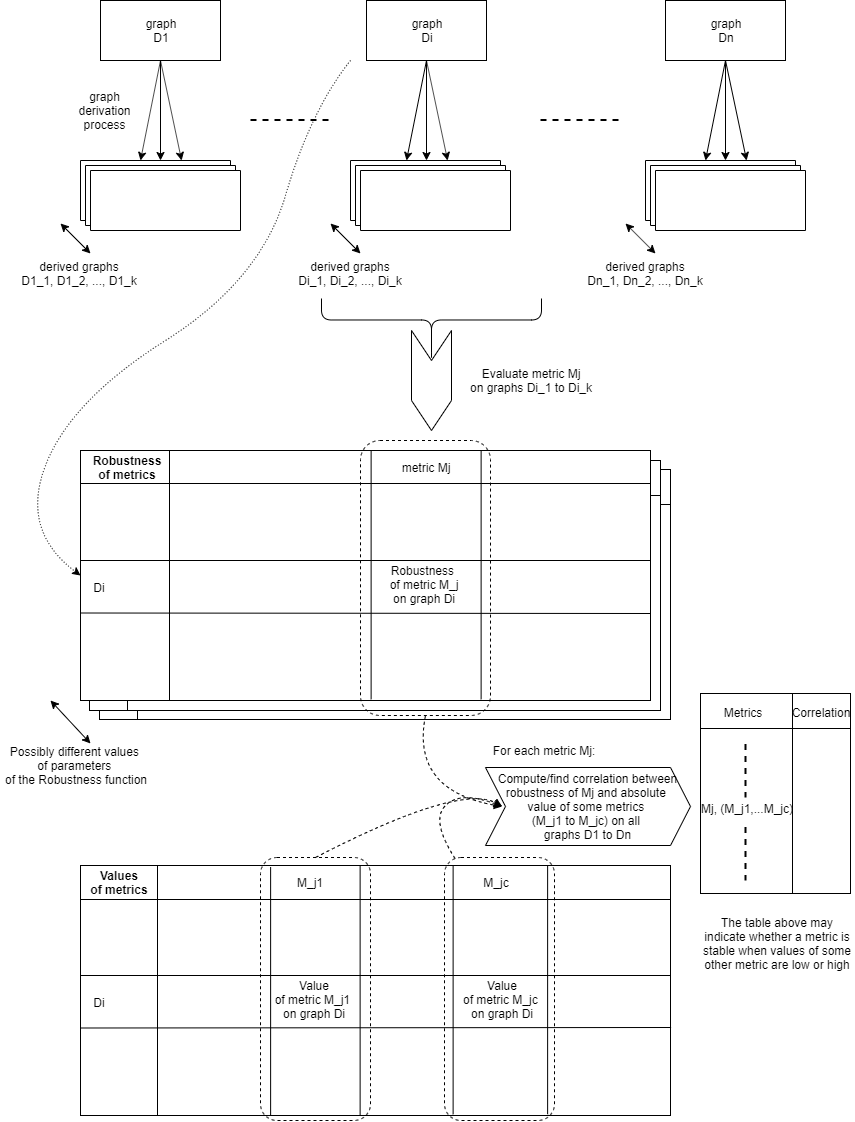
\includegraphics[width=16cm]{images/proposal_diagram1.png}
            \caption{An example of the evaluation process}
			\label{fig:example_eval}
            \end{figure}
	
	%I intend to use the programming language \textbf{Kotlin}, mainly for the following reasons. It is by nature similar to Java and can be used together with other Java code in a single project. Performance-wise, Kotlin is comparable to Java.
	%\begin{itemize}
	%    \item Concise, reducing the amount of boilerplate code
	%    \item Safe, preventing a significant number of errors
	%    \item IDE-friendly, allowing the IDE to help with software engineering
	%    \item Allows more functional constructs than Java
	%    \item Compiles to Java byte code and so preserves other important benefits of Java: Object-Oriented, platform-independent, extensible.
	%\end{itemize}
	
	\subsection*{Tasks}
	
	The following tasks need to be carried out to complete this project to the state described above.
	
	\begin{enumerate}
		
		\item Decide on the underlying graph framework, the programming language, tools and additional libraries to use for developing the software.
		
		\item Study graphs and their metrics to decide which metrics to carry out the described experiment on. This may depend on the complexity of the algorithm of the metric, usefulness of the metric in the graph research context, computing feasibility to evaluate the metric on large datasets and other factors.
		
		\item Study possible graph datasets and decide which graphs will be used in the experiment. Again this will take into account multiple factors such as availability of such datasets, commonness of the respective application area and others. This project intends to study robustness of graph metrics on graphs from different application areas.
		
		\item Devise a 'robustness' measure of a metric applied to a graph (possibly more measures for different aspects of robustness). This will likely be a function of a metric and an input graph, and will likely involve generating multiple graphs from the input graph that the robustness will be calculated for, for example by randomly deleting a small percentage of edges. For this, I will need to decide on what 'small perturbations' mean, which may as well be left as a parameter of the robustness measure.
		
		\item Build the platform to do the following:
		\begin{itemize}
		    \item Store, load and represent input graphs
		    \item Implement (or integrate existing) algorithms to compute graph metrics
		    \item Generate similar graphs, given an input graph, by making small changes or deletions
		    \item Implement the robustness function
		    \item Possibly, if suitable, produce visual results directly from the program
		\end{itemize}
		
		\item Execute the result, i.e. compute the robustness function value for chosen graph metrics and chosen input graphs, trying different values of parameters if appropriate.
		
		\item Evaluate the outcome and conclude the findings. Compare graph metrics in terms of their robustness based on the results of the experiment. Possibly compare the results of this experiment to the results of the paper by Bozhilova et al.
		
		\item Write up the dissertation.
		
	\end{enumerate}
	
	This project may additionally involve the use of secondary languages and platforms (such as Python, Jupyter notebook) for statistical analysis etc.

\section*{Success criteria}

	This project will be considered a success if I manage to complete the steps described above, primarily to execute the experiment and conclude any observations about graph metrics.
	
	\begin{enumerate}
	    \item Implement the experimental framework outlined above, using interesting datasets
	    \item Complete statistical analysis, as described in the~\nameref{evaluation} section
	    \item Deduce empirical observations about graph metrics
	\end{enumerate}
	
	The results of the experiment may also be compared to the results of the originating paper by Bozhilova, L. V., et al.

\section*{Possible extensions}

    The following ideas could be developed in case there is spare time during the implementation phase.
    
    \begin{enumerate}
        \item Wrap up and publish the project as an open-source library that can further be used by future projects.
        \item Develop a plugin to the Gephi graph visualisation software, to compute robustness of different metrics within the Gephi user interface.
        \item Produce a program, that will, given an input graph, be able to advise which metrics are more suited for describing such graph
    \end{enumerate}

\section*{Timetable}

	Planned starting date is 28 October 2019.
	
	\subsection*{Weeks 1 to 2}
	
		Research and read papers on similar topics. Read about graphs and network from relevant books.
		
		\textit{Milestone \textbf{8 November}: Fully understand the problem this project is solving and approaches possible.}
	
	\subsection*{Weeks 3 to 4}
	
	    Set up the working environment, decide on programming language and tools needed, repositories for code and dissertation, find and integrate relevant libraries, familiarise myself by creating toy programs on graphs.
	    
	    By taking various factors into account, decide on which metrics to analyse and which graph datasets to choose for the experiment. Use toy programs to estimate the complexity and feasibility of different algorithms on the datasets.
	    
	    \textit{Milestone \textbf{22 November}: Have a fully working setup of the programming environment with backup plans.}
		
	\subsection*{Weeks 5 to 6}
	
	    Devise the robustness measure(s) and mathematics behind the experiment. Write up the beginning of the dissertation.
	    
	    Beginning of the implementation: storing, loading and representing input graphs. Also, be able to generate pseudo-random graphs derived from an input graph.
	    
	    \textit{Milestone 6 December: Fully understand what robustness function the program will calculate and how.}
	
	\subsection*{Weeks 7 to 8}
	
	    Implement algorithms of the metrics to evaluate. Document the implementation.
	
		\textit{Milestone \textbf{20 December}: Working algorithm for each chosen metric}
		
    \subsection*{Weeks 9 to 10}
	
		Winter break, no work planned.
		
		%\textit{Milestone 3 January:}
	
	\subsection*{Weeks 11 to 12}
	
		Start implementation of the robustness measure(s).
		
		%\textit{Milestone \textbf{17 January}: }
		
	\subsection*{Weeks 13 to 14}
	
		Finish implementing the robustness measure(s) and a way to compare metrics. Write the Progress Report.
		
		\textit{Milestone \textbf{31 January}: Be able to calculate the robustness measure, for a given collection of similar graphs and a graph metric. Submit the Progress Report.}
	
	\subsection*{Weeks 15 to 16}
	
		Refine the robustness measure implementation. Integrate the individual parts of the implementation to create an executable program taking input parameters. If suitable, produce a statistical output from the program.
		
		\textit{Milestone \textbf{14 February}: Executable program}

	\subsection*{Weeks 17 to 18}
		
		Execute the evaluation (this may be very computationally expensive). Compare individual metrics and conclude results. Start writing the dissertation.
		
		\textit{Milestone \textbf{28 February}: Have some results of the evaluation}

	\subsection*{Weeks 19 to 20}
	
		Continue with carrying out the experiment. Over this period, focus mainly on writing the dissertation.
		
		%\textit{Milestone 13 March: Have some output}
	
	\subsection*{Weeks 21 to 22}
	
		Finish evaluation. Conclude experiment results. Continue writing the dissertation.
		
		\textit{Milestone \textbf{27 March}: Have the majority of the dissertation written up.}
	
	\subsection*{Weeks 23 to 24}
	
	    Ideally, work on extensions, or finish the implementation/evaluation if needed. Collect thorough feedback on the dissertation.
		
		\textit{Milestone \textbf{10 April}: Have a finished dissertation.}
	
	\subsection*{Weeks 25 to 26}
		
		The dissertation should be done by now. Polishing of the work if needed.
		
		%\textit{Milestone 24 April:}
		
	\subsection*{Weeks 27 to 28}
	
	    No work planned.
	    
	    \textit{Milestone \textbf{8 May}: Submit the dissertation}

\section*{Resource Declaration} \label{resourceDeclaration}

    \subsection*{Personal resources}

    For the development and writing the dissertation, I will primarily use my personal laptop with an IDE such as IntelliJ IDEA. Source code and the written work will regularly be version-controlled in a git repository, backed up on GitHub and possibly other relevant online storage places. I accept full responsibility for this machine and the software and I have made contingency plans to protect myself against hardware and/or software failure, such as to fallback to using the MCS computers.

    \subsection*{Computing resources}

    This project requires the use of a high-performance computing resource, to run algorithms of evaluating metrics and their robustness on large (real-world or derived) graphs.
    
    Based on the paper by Bozhilova et al., calculating natural connectivity for a single node for a graph with ~7000 nodes takes ~88 seconds on a standard computer. Based on my toy example, calculating average betweenness centrality of ~2500 nodes takes ~8 minutes on my computer. Thus, assuming that computing a metric for an input graph of average size 5000 nodes takes ~1 hour, the pure computation time suggested by this Project Proposal would take the following time on a standard personal computer (approximated in the order of magnitude)
    \[(\sim 6\ \text{datasets}) \times (\sim 6\ \text{metrics}) \times (\sim 50\ \text{derived graphs}) \times (\sim 1\ \text{hour}) \approx 75\ \text{days}\]
    
    The following resource has been granted permission for and will be used to parallelise the process and thus significantly speed up the computation time:
    
    \begin{adjustwidth}{1cm}{}
    	Resource: a computing facility (such as one of the servers \textit{yellow, nile,} or \textit{rio})\\
    	Institution: Systems Research Group (\url{https://www.cl.cam.ac.uk/research/srg/})\\
    	Sponsor: Dr Andrew Moore (\url{andrew.moore@cl.cam.ac.uk})
    	
    	This requires setting up a Computer Laborarory account.
	\end{adjustwidth}
    
    An alternative to this is Amazon Web Services or Google Cloud with free credits for students.
    
    \subsection*{Datasets}
    
    Graph datasets are available and will be obtained from either of the following sources (or others):
    
    \begin{itemize}
        \item Stanford Large Network Dataset Collection: \url{https://snap.stanford.edu/data/}
        \item STRING Database: \url{https://string-db.org/}
    \end{itemize}

\end{document}


    %TC:endignore
\end{document}
